% Compilador en Overleaf: pdfLaTeX (el que viene por defecto)
% Manual: Seguridad Operacional y Gestión en Operaciones Aéreas
%         Entorno: Legislación Aeronáutica — 7mo año, Técnico/a en Aviónica
\documentclass[11pt,a4paper,oneside]{article}
\usepackage[T1]{fontenc}
\usepackage[utf8]{inputenc}
\IfFileExists{spanish.ldf}{\usepackage[spanish,es-noshorthands]{babel}}{}
\usepackage{lmodern} % tipografía estándar de LaTeX (Computer Modern)
\usepackage[a4paper,top=3cm,bottom=2.5cm,left=2.5cm,right=2cm,headheight=15pt,footskip=1.1cm]{geometry}
\usepackage{graphicx}
\usepackage{tikz}
\usetikzlibrary{arrows.meta,positioning,shapes.geometric}
\usepackage{xcolor}
\usepackage{enumitem}
\usepackage{fancyhdr}
\usepackage{microtype}
\usepackage{array}
\usepackage{titlesec}
\usepackage[most]{tcolorbox}

% ---------- Formato general
\setlength{\parindent}{0pt}
\setlength{\parskip}{4pt}
\setlist[itemize]{itemsep=1pt,topsep=2pt,parsep=0pt}
\setlist[enumerate]{itemsep=1pt,topsep=2pt,parsep=0pt}
\renewcommand{\arraystretch}{1.15}
\newtcolorbox{recuadro}{enhanced,breakable,colback=white,colframe=black,
  boxrule=0.6pt,arc=0pt,left=5pt,right=5pt,top=3pt,bottom=3pt}
\titleformat{\section}{\large\bfseries\centering}{}{0pt}{}
\titleformat{\subsection}{\large\bfseries\itshape\centering}{}{0pt}{\underline}
\titleformat{\subsubsection}{\normalsize\bfseries}{}{0pt}{}
\titlespacing*{\section}{0pt}{14pt}{8pt}
\titlespacing*{\subsection}{0pt}{12pt}{6pt}
\titlespacing*{\subsubsection}{0pt}{10pt}{3pt}
\titlespacing*{\paragraph}{0pt}{6pt}{0.6em}
\newcommand{\casilla}{\raisebox{-0.12em}{\tikz\draw[thick] (0,0) rectangle (0.34,0.34);}}

% ---------- Encabezado y pie (mismo diseño que el manual de Emprendimientos)
\definecolor{ppAzul}{rgb}{0.267,0.447,0.769}
\definecolor{ppAzulClaro}{rgb}{0.557,0.667,0.859}
\fancypagestyle{materia}{%
  \fancyhf{}%
  \fancyhead[L]{\color{ppAzul}\bfseries\itshape 7mo Año}%
  \fancyhead[R]{\color{ppAzul}\bfseries\itshape Seguridad Operacional y Gestión}%
  \fancyfoot[L]{\small\color{ppAzulClaro}\itshape scicolonejulian@impatrq.com}%
  \fancyfoot[C]{\raisebox{-0.7\height}{
\includegraphics[height=0.8cm]{logos/logo-impa}}}%
  \fancyfoot[R]{\small\color{ppAzulClaro}\itshape\thepage}%
  \renewcommand{\headrule}{{\color{ppAzul}\hrule height 0.5pt}}%
  \renewcommand{\footrule}{{\color{ppAzul}\hrule height 0.5pt}\vspace{2pt}}%
}

\begin{document}
% ============================================================
% Carátula — reemplaza el bloque \begin{titlepage}...\end{titlepage}
% Requiere en el preámbulo: \usepackage{graphicx} y \usepackage{tikz}
% Logos en la carpeta logos/ (logo-impa.pdf y logo-pba.pdf)
% ============================================================
\begin{titlepage}
% Logo PBA en el margen superior derecho (posición absoluta en la hoja)
\begin{tikzpicture}[remember picture,overlay]
  \node[anchor=north east,inner sep=0pt]
    at ([xshift=-1.5cm,yshift=-1.2cm]current page.north east)
    {
\includegraphics[width=9.75cm]{logos/logo-pba}};
\end{tikzpicture}

\centering
\vspace*{2.58cm}
% Títulos superiores del logo IMPA
{\fontsize{20.74}{25}\selectfont\bfseries Escuela de Educación Secundaria Técnica\par}
\vspace{0.2cm}
{\fontsize{20.74}{25}\selectfont\bfseries N° 7 - Quilmes\par}
\vspace{0.5cm}
% Logo IMPA centrado y grande

\includegraphics[width=0.775\linewidth]{logos/logo-impa}\par
\vspace{0.4cm}
% Título inferior del logo IMPA
{\fontsize{20.74}{25}\selectfont\bfseries Taller Regional Quilmes\par}
\vspace{1.4cm}
\fbox{\parbox{0.8\linewidth}{\centering\vspace{1em}
{\fontsize{24.88}{30}\selectfont\bfseries SEGURIDAD\\ OPERACIONAL Y\\ GESTIÓN EN\\ OPERACIONES AÉREAS\par}\vspace{0.6em}
{\fontsize{17.28}{21}\selectfont\bfseries\itshape Entorno: Legislación Aeronáutica\par}\vspace{1em}}}\par
\vspace{0.8cm}
% Año / curso
{\fontsize{20.74}{25}\selectfont\bfseries 7mo año\par}
\vfill
{\fontsize{14.4}{17.3}\selectfont\bfseries EDICIÓN\par}
\vspace{0.2cm}
{\fontsize{14.4}{17.3}\selectfont\bfseries CICLO LECTIVO 2026\par}
\end{titlepage}

\pagestyle{materia}
\setcounter{page}{2}
% ============================================================
% PRESENTACIÓN DE LA MATERIA
% ============================================================
\section*{PRESENTACIÓN DE LA MATERIA}
\subsection*{Seguridad Operacional y Gestión en Operaciones Aéreas}

\begin{center}
\small
\begin{tabular}{|p{0.32\linewidth}|p{0.58\linewidth}|}
\hline
\textbf{Escuela} & E.E.S.T. N° 7 ``Taller Regional Quilmes'' (IMPA) \\ \hline
\textbf{Especialidad} & Técnico/a en Aviónica \\ \hline
\textbf{Año} & 7mo año \\ \hline
\textbf{Campo} & Formación Científico Tecnológica \\ \hline
\textbf{Módulo} & Seguridad Operacional y Gestión en Operaciones Aéreas \\ \hline
\textbf{Entorno} & Legislación Aeronáutica \\ \hline
\textbf{Carga horaria} & 4 horas semanales -- 144 horas anuales \\ \hline
\textbf{Marco curricular} & Diseño Curricular 2025 de la Educación Secundaria Técnica, Provincia de
Buenos Aires \\ \hline
\textbf{Docente} & Téc. Aviónico Julián Scicolone -- scicolonejulian@impatrq.com \\ \hline
\end{tabular}
\end{center}

% ------------------------------------------------------------
\section*{FUNDAMENTACIÓN}

Un técnico aviónico no solo repara equipos: trabaja dentro de un sistema regulado, firma
documentos con valor legal y forma parte de organizaciones donde un error puede costar vidas. Por
eso el Diseño Curricular propone en este módulo el análisis integral de la \textbf{gestión de los
recursos humanos en organizaciones aéreas}, reconociendo la actuación humana como un factor
crítico en la operación y el mantenimiento, el estudio del \textbf{marco legal vigente} (Código
Aeronáutico, anexos de la OACI y regulaciones del Estado que rigen las licencias), el
\textbf{rol del técnico como representante técnico} de los talleres y la \textbf{oficina técnica}
como ámbito profesional, y la \textbf{prevención de accidentes} mediante las mejores prácticas
de gestión de la seguridad operacional.

\begin{recuadro}
\textbf{Un dato que le da sentido a esta materia.} Desde la Resolución ANAC N° 443/2025, el
\textbf{título de Técnico en Aviónica emitido por una escuela técnica} es uno de los títulos
aceptados para solicitar la \textbf{licencia de Mecánico de Equipos Radioeléctricos de Aeronaves
(MERA)}. Todo lo que se estudia en este manual (las regulaciones, la documentación, los factores
humanos y la seguridad operacional) es lo que se espera de un titular de esa licencia.
\end{recuadro}

% ------------------------------------------------------------
\section*{OBJETIVOS DE APRENDIZAJE}
Según el Diseño Curricular 2025, al finalizar el módulo se espera que las y los estudiantes
puedan:
\begin{itemize}
  \item Utilizar conceptos, herramientas, métodos y técnicas de la \textbf{gestión
        organizacional} de una empresa del ámbito aeronáutico en cualquiera de sus formas.
  \item Utilizar conceptos, herramientas, métodos y técnicas de la \textbf{gestión de calidad e
        impacto ambiental}.
  \item Utilizar conceptos, herramientas, métodos y técnicas de la \textbf{gestión de los
        recursos humanos} a través de programas de CRM o MRM.
  \item Interrelacionar la gestión global y la gestión de sus actividades específicas.
  \item Comprender el proceso productivo y la estructura organizacional de una empresa del sector
        aeronáutico (comercialización, selección y abastecimiento de sistemas, componentes y
        partes), en el marco de la normativa aeronáutica nacional e internacional vigente.
  \item Planificar, programar y organizar la producción, la prestación de servicios y el
        mantenimiento.
  \item \textbf{Planificar y gestionar un SMS} en un taller u organización aeronáutica.
  \item Identificar proyectos productivos y de servicio, evaluar su factibilidad
        técnico-económica, programar su implementación y su gestión.
\end{itemize}

% ------------------------------------------------------------
\section*{ORGANIZACIÓN DEL MANUAL}

\begin{center}
\small
\begin{tabular}{|c|>{\raggedright\arraybackslash}p{0.48\linewidth}|>{\raggedright\arraybackslash}p{0.33\linewidth}|}
\hline
\textbf{Unidad} & \textbf{Contenidos} & \textbf{Bloque del Diseño Curricular} \\ \hline
1 & Derecho aeronáutico: OACI, Código Aeronáutico, ANAC, JST, RAAC. Rol regulador del Estado. &
Derecho aeronáutico y aeronavegabilidad \\ \hline
2 & Aeronavegabilidad y certificación: aeronaves, partes, documentación, ATA 100/104, normas ISO,
AN, MS, NAS, MIL. & Derecho aeronáutico y aeronavegabilidad \\ \hline
3 & Licencias del personal (RAAC 65), representante técnico y oficina técnica. & Derecho
aeronáutico y aeronavegabilidad; Oficina técnica \\ \hline
4 & Organizaciones aeronáuticas: talleres, operadores, planificación del mantenimiento,
abastecimiento, control de gestión, economía del operador, calidad, ambiente y salud laboral. &
Organizaciones aeronáuticas \\ \hline
5 & Actuación humana: factores humanos, error humano, MRM, MEDA, reportes, primeros auxilios. &
Actuación humana \\ \hline
6 & Prevención de accidentes: riesgo, causalidad, investigación, SMS, costos de la seguridad
operacional, casos reales. & Prevención de accidentes \\ \hline
7 & Operaciones aéreas: tipos de operación, espacio aéreo y cartas aeronáuticas. &
Complementario \\ \hline
PI & Proyecto integrador: SMS del taller de aviónica de la escuela. & Prácticas formativas \\
\hline
\end{tabular}
\end{center}

\paragraph*{Metodología.} Cada unidad combina explicación teórica, lectura de normativa real,
análisis de casos (accidentes e incidentes investigados) y prácticas formativas en el taller.
Al final de cada unidad hay actividades. El año cierra con un \textbf{proyecto integrador}: el
diseño e implementación de un Sistema de Gestión de la Seguridad Operacional (SMS) para el
taller de la escuela.

\paragraph*{Fuentes.} Las regulaciones aeronáuticas cambian con frecuencia. Este manual está
actualizado a noviembre de 2026; antes de usar un dato normativo en un trabajo real, verificar
siempre la versión vigente en el sitio de la ANAC (\texttt{argentina.gob.ar/anac}) y en el
Boletín Oficial.

% ------------------------------------------------------------
\clearpage
\section*{HOJA DE RUTA DEL ESTUDIANTE}
\subsection*{Lo que vas a tener hecho al terminar el año}

\vspace{2pt}
{\small
\renewcommand{\arraystretch}{1.3}
\begin{tabular}{|c|>{\raggedright\arraybackslash}p{0.54\linewidth}|>{\centering\arraybackslash}p{0.08\linewidth}|>{\centering\arraybackslash}p{0.17\linewidth}|}
\hline
\textbf{OK} & \textbf{Logro} & \textbf{Unidad} & \textbf{Firma docente} \\ \hline
\casilla & Esquema institucional del sistema aeronáutico argentino (OACI, ANAC, JST, EANA, ORSNA) &
1 & \\ \hline
\casilla & Cuadro comparativo de normativa nacional e internacional & 1 & \\ \hline
\casilla & Verificación simulada de la aeronavegabilidad de una aeronave (documentos a bordo,
AD, registros) & 2 & \\ \hline
\casilla & Búsqueda de una tarea en un manual por capítulo ATA y de una parte en el IPC & 2 & \\
\hline
\casilla & Tabla comparativa de normas ISO, AN, MS, NAS y MIL & 2 & \\ \hline
\casilla & Carpeta de solicitud simulada de la licencia MERA & 3 & \\ \hline
\casilla & Organigrama funcional de un TAR con el rol del representante técnico & 3 & \\ \hline
\casilla & Registro de mantenimiento y retorno al servicio completados & 3 & \\ \hline
\casilla & Plan de mantenimiento e indicadores de gestión de una flota simulada & 4 & \\ \hline
\casilla & Caso práctico de economía del operador (costo de mantenimiento por hora de vuelo) & 4
& \\ \hline
\casilla & Simulación de pase de turno con planilla MRM & 5 & \\ \hline
\casilla & Reporte e investigación de un error con el método MEDA & 5 & \\ \hline
\casilla & Práctica de primeros auxilios (RCP y control de hemorragias) & 5 & \\ \hline
\casilla & Análisis de un accidente real con el modelo de Reason & 6 & \\ \hline
\casilla & Matriz de riesgos del taller de la escuela & 6 & \\ \hline
\casilla & Informe que justifique una inversión en prevención & 6 & \\ \hline
\casilla & Lectura de una carta aeronáutica y de un NOTAM & 7 & \\ \hline
\casilla & Proyecto integrador: manual SMS del taller presentado & PI & \\ \hline
\end{tabular}
}

\vspace{8pt}
\noindent Estudiante: \dotfill \quad Curso: \makebox[3cm]{\dotfill}

\vspace{6pt}
\noindent Logros completados: \makebox[1.5cm]{\dotfill} de 18 \hfill Fecha: \makebox[4cm]{\dotfill}
      % Fundamentación, objetivos, organización y hoja de ruta
% ============================================================
% UNIDAD 1: DERECHO AERONÁUTICO Y ROL REGULADOR DEL ESTADO
% ============================================================
\clearpage
\section*{UNIDAD 1: DERECHO AERONÁUTICO}
\subsection*{Marco internacional, marco nacional y rol regulador del Estado}

\begin{recuadro}
\textbf{Objetivo de la unidad:} conocer de dónde salen las reglas que rigen la aviación, quién
las dicta y quién controla que se cumplan, tanto a nivel internacional (OACI) como nacional
(Código Aeronáutico, ANAC, JST, RAAC), y ubicar el lugar del técnico aeronáutico dentro de ese
sistema.
\end{recuadro}

% ------------------------------------------------------------
\section*{1. ¿QUÉ ES EL DERECHO AERONÁUTICO?}

El \textbf{derecho aeronáutico} es el conjunto de normas, nacionales e internacionales, que
regulan la actividad aeronáutica: la circulación de aeronaves, la infraestructura (aeródromos,
servicios de navegación aérea), las aeronaves y su aeronavegabilidad, el personal aeronáutico y
sus licencias, el transporte de pasajeros y carga, la responsabilidad por daños y la
investigación de accidentes.

\subsubsection*{1.1. Características}
\begin{itemize}
  \item \textbf{Internacional:} un avión cruza fronteras en minutos; las reglas tienen que ser
        parecidas en todos los países. Por eso gran parte de las normas nacionales copian las
        normas de la OACI.
  \item \textbf{Dinámico:} la tecnología cambia rápido (motores a reacción, GPS, drones) y las
        normas se actualizan constantemente.
  \item \textbf{Autónomo:} tiene principios propios, distintos del derecho marítimo o del
        terrestre.
  \item \textbf{Integral:} mezcla derecho público (Estado, autoridad, sanciones) y privado
        (contratos de transporte, seguros, responsabilidad).
  \item \textbf{Técnico:} muchas de sus normas son reglas técnicas (cómo se mantiene un avión,
        qué instrumentos debe llevar, cuántas horas puede trabajar un tripulante).
\end{itemize}

\subsubsection*{1.2. Fuentes}
\begin{center}
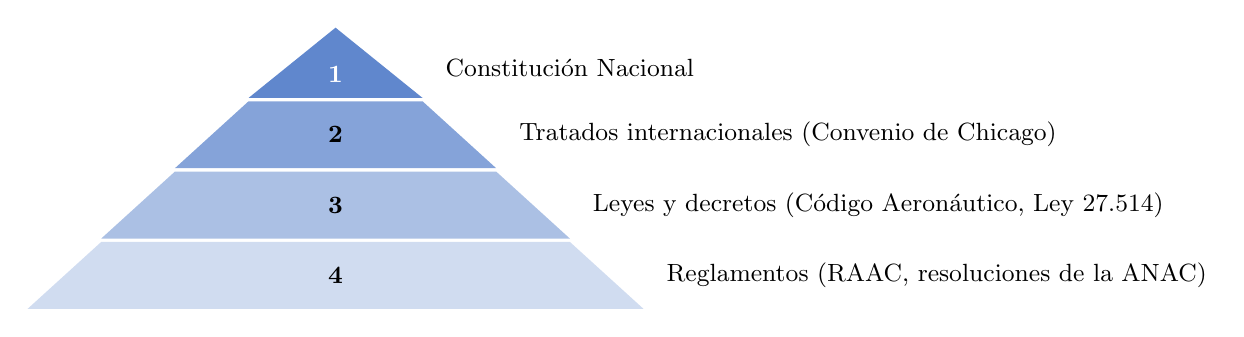
\begin{tikzpicture}[scale=0.85, every node/.style={font=\small, align=center}]
  \fill[ppAzul!85] (0,4.2) -- (-1.3,3.15) -- (1.3,3.15) -- cycle;
  \node[white] at (0,3.5) {\textbf{1}};
  \fill[ppAzul!65] (-1.3,3.1) -- (1.3,3.1) -- (2.4,2.1) -- (-2.4,2.1) -- cycle;
  \fill[ppAzul!45] (-2.4,2.05) -- (2.4,2.05) -- (3.5,1.05) -- (-3.5,1.05) -- cycle;
  \fill[ppAzul!25] (-3.5,1.0) -- (3.5,1.0) -- (4.6,0) -- (-4.6,0) -- cycle;
  \node at (0,2.6) {\textbf{2}};
  \node at (0,1.55) {\textbf{3}};
  \node at (0,0.5) {\textbf{4}};
  \node[anchor=west] at (1.5,3.6) {Constitución Nacional};
  \node[anchor=west] at (2.6,2.6) {Tratados internacionales (Convenio de Chicago)};
  \node[anchor=west] at (3.7,1.55) {Leyes y decretos (Código Aeronáutico, Ley 27.514)};
  \node[anchor=west] at (4.8,0.5) {Reglamentos (RAAC, resoluciones de la ANAC)};
\end{tikzpicture}
\end{center}
A estas fuentes escritas se suman la \textbf{costumbre} (prácticas aceptadas de la industria),
la \textbf{jurisprudencia} (fallos judiciales) y la \textbf{doctrina} (estudios de juristas).
Además, los documentos técnicos de los fabricantes y de la OACI funcionan en la práctica como
``normas'' de cumplimiento obligatorio cuando una regulación los incorpora.

% ------------------------------------------------------------
\section*{2. EL MARCO INTERNACIONAL}

\subsubsection*{2.1. Antecedentes}
\begin{itemize}
  \item \textbf{Convención de París (1919):} primer gran tratado; reconoció que cada Estado es
        soberano sobre el espacio aéreo que cubre su territorio.
  \item \textbf{Convenio de Varsovia (1929):} reguló la responsabilidad del transportista aéreo
        internacional por daños a pasajeros y equipajes. Hoy lo reemplaza, para la mayoría de
        los países, el \textbf{Convenio de Montreal (1999)}.
  \item \textbf{Convenio de Chicago (1944):} es la ``constitución'' de la aviación civil
        internacional.
\end{itemize}

\subsubsection*{2.2. El Convenio sobre Aviación Civil Internacional (Chicago, 1944)}
Firmado el 7 de diciembre de 1944, mientras terminaba la Segunda Guerra Mundial. La Argentina lo
aprobó por la \textbf{Ley 13.891}. Sus principios más importantes:
\begin{itemize}
  \item \textbf{Soberanía:} cada Estado tiene soberanía plena y exclusiva sobre el espacio aéreo
        situado sobre su territorio (artículo 1).
  \item \textbf{Nacionalidad de las aeronaves:} toda aeronave tiene la nacionalidad del Estado
        en que está matriculada, y solo puede estar matriculada en un Estado.
  \item \textbf{Documentos a bordo:} toda aeronave en vuelo internacional debe llevar, entre
        otros, su \textbf{certificado de matrícula}, su \textbf{certificado de
        aeronavegabilidad} y las \textbf{licencias} de la tripulación.
  \item \textbf{Reconocimiento mutuo:} los certificados de aeronavegabilidad y las licencias
        emitidos por un Estado son reconocidos por los demás, siempre que cumplan como mínimo
        las normas de la OACI.
  \item \textbf{Creación de la OACI}, que comenzó a funcionar en 1947.
\end{itemize}

\paragraph*{Las libertades del aire.}
Son los derechos que los Estados se conceden entre sí para operar vuelos comerciales:
\begin{center}
\small
\begin{tabular}{|c|p{0.80\linewidth}|}
\hline
\textbf{Libertad} & \textbf{Derecho} \\ \hline
1.ª & Sobrevolar el territorio de otro Estado sin aterrizar. \\ \hline
2.ª & Aterrizar en otro Estado con fines no comerciales (combustible, mantenimiento). \\ \hline
3.ª & Llevar pasajeros o carga desde el propio país hacia otro país. \\ \hline
4.ª & Traer pasajeros o carga desde otro país hacia el propio. \\ \hline
5.ª & Llevar pasajeros entre dos países extranjeros, en un vuelo que empieza o termina en el
propio país. \\ \hline
6.ª a 9.ª & Combinaciones más amplias, incluido el \textbf{cabotaje} (vuelos internos en otro
país), que muy pocos Estados conceden. \\ \hline
\end{tabular}
\end{center}

\subsubsection*{2.3. La OACI}
La \textbf{Organización de Aviación Civil Internacional} (OACI, en inglés ICAO) es un organismo
especializado de las Naciones Unidas, con sede en Montreal (Canadá), del que forman parte casi
todos los países del mundo.
\begin{itemize}
  \item \textbf{Asamblea:} todos los Estados; se reúne cada tres años.
  \item \textbf{Consejo:} órgano ejecutivo permanente; adopta las normas.
  \item \textbf{Comisión de Aeronavegación:} estudia y propone las normas técnicas.
  \item \textbf{Secretaría} y \textbf{oficinas regionales} (la Argentina depende de la Oficina
        Sudamericana, en Lima).
\end{itemize}

\paragraph*{SARPs: normas y métodos recomendados.}
La OACI dicta \textbf{SARPs} (\textit{Standards and Recommended Practices}):
\begin{itemize}
  \item \textbf{Norma:} su aplicación uniforme es \textbf{necesaria}. Si un Estado no la puede
        cumplir, debe \textbf{notificar la diferencia} a la OACI.
  \item \textbf{Método recomendado:} su aplicación es \textbf{conveniente}; los Estados procuran
        cumplirlo.
\end{itemize}
Los SARPs se publican en los \textbf{19 Anexos} al Convenio, y se complementan con
\textbf{documentos} (manuales) que explican cómo aplicarlos, como el Doc 9859, \textit{Manual de
gestión de la seguridad operacional}.

\begin{center}
\small
\begin{tabular}{|c|p{0.36\linewidth}||c|p{0.36\linewidth}|}
\hline
\textbf{Anexo} & \textbf{Tema} & \textbf{Anexo} & \textbf{Tema} \\ \hline
1 & \textbf{Licencias al personal} & 11 & Servicios de tránsito aéreo \\ \hline
2 & Reglamento del aire & 12 & Búsqueda y salvamento \\ \hline
3 & Meteorología & 13 & \textbf{Investigación de accidentes e incidentes} \\ \hline
4 & Cartas aeronáuticas & 14 & Aeródromos \\ \hline
5 & Unidades de medida & 15 & Servicios de información aeronáutica \\ \hline
6 & \textbf{Operación de aeronaves} & 16 & Protección del medio ambiente \\ \hline
7 & Marcas de nacionalidad y matrícula & 17 & Seguridad (protección contra actos de
interferencia ilícita) \\ \hline
8 & \textbf{Aeronavegabilidad} & 18 & Mercancías peligrosas \\ \hline
9 & Facilitación & 19 & \textbf{Gestión de la seguridad operacional} \\ \hline
10 & Telecomunicaciones aeronáuticas (incluye radioayudas y comunicaciones: el corazón de la
aviónica) & & \\ \hline
\end{tabular}
\end{center}

\paragraph*{Auditorías.}
La OACI audita a los Estados mediante el \textbf{USOAP} (Programa universal de auditoría de la
vigilancia de la seguridad operacional), que mide si cada país tiene la capacidad de controlar
eficazmente su aviación civil.

\subsubsection*{2.4. Otras autoridades de referencia}
\begin{itemize}
  \item \textbf{FAA} (Administración Federal de Aviación, EE.\,UU.): sus regulaciones (\textbf{FAR},
        14 CFR) son la base histórica de las RAAC, y la mayor parte de la flota argentina es de
        diseño estadounidense.
  \item \textbf{EASA} (Agencia de la Unión Europea para la Seguridad Aérea): autoridad europea;
        certifica a Airbus y a muchos fabricantes de equipos.
  \item \textbf{SRVSOP} (Sistema Regional de Cooperación para la Vigilancia de la Seguridad
        Operacional): sistema de cooperación de los países sudamericanos, que elabora los
        \textbf{LAR} (Reglamentos Aeronáuticos Latinoamericanos) para armonizar las normas de la
        región.
\end{itemize}

\begin{recuadro}
\textbf{Seguridad operacional (\textit{safety}) y seguridad de la aviación (\textit{security}).}
En español usamos ``seguridad'' para dos cosas distintas. La \textbf{seguridad operacional}
(\textit{safety}) trata de evitar accidentes por fallas técnicas, errores humanos o
condiciones peligrosas: es el tema de esta materia (Anexos 6, 8, 13 y 19). La \textbf{seguridad
de la aviación} o protección (\textit{security}, AVSEC) trata de evitar actos de interferencia
ilícita: secuestros, sabotajes, terrorismo (Anexo 17); en la Argentina la ejerce, entre otros,
la Policía de Seguridad Aeroportuaria.
\end{recuadro}

% ------------------------------------------------------------
\section*{3. EL MARCO NACIONAL}

\subsubsection*{3.1. El Código Aeronáutico (Ley 17.285)}
Sancionado en 1967, es la ley que rige la aeronáutica civil en el territorio argentino, su mar
territorial y el espacio aéreo que los cubre. Trata, entre otros temas:
\begin{itemize}
  \item la circulación aérea y la infraestructura (aeródromos, servicios);
  \item las \textbf{aeronaves}: definición, nacionalidad, \textbf{Registro Nacional de Aeronaves},
        matrícula, certificado de aeronavegabilidad;
  \item el \textbf{personal aeronáutico}: necesita una licencia o certificado de idoneidad
        expedido por la autoridad para ejercer sus funciones;
  \item la explotación comercial y el contrato de transporte aéreo;
  \item la responsabilidad por daños a pasajeros, cargas y terceros en la superficie;
  \item la búsqueda, asistencia y salvamento, y la investigación de accidentes;
  \item las faltas, delitos y sanciones.
\end{itemize}

\paragraph*{Reformas recientes.}
Entre 2023 y 2025 el Código fue modificado varias veces por decretos de necesidad y urgencia
(DNU 70/2023, 941/2024 y 338/2025), con el objetivo declarado de desregular la actividad
aerocomercial: apertura del mercado a nuevas empresas y rutas (``cielos abiertos''),
simplificación de trámites, eliminación de requisitos considerados obsoletos y posibilidad de
que la autoridad delegue algunas funciones de certificación en personas habilitadas. También se
calificó a la aeronáutica civil aerocomercial como \textbf{servicio esencial}. Las reformas son
objeto de debate entre quienes destacan la mayor competencia y quienes advierten sobre sus
efectos en el empleo y en la vigilancia estatal; para esta materia lo importante es saber que
\textbf{las normas cambian} y que hay que trabajar siempre con la versión vigente.

\subsubsection*{3.2. Los organismos del sistema aeronáutico argentino}
% Logos: colocar los archivos en logos/organismos/ con estos nombres (png, jpg o pdf):
% transporte, anac, jst, eana, orsna, psa, fuerza_aerea (Fuerza Aérea Argentina), smn.
% Si un archivo no está, se muestra un recuadro con la sigla.
\newcommand{\logoorg}[2]{\vspace{2pt}\logoorgimg{#1}{#2}\vspace{2pt}}
\newcommand{\logoorgimg}[2]{%
  \IfFileExists{logos/organismos/#1.png}{\includegraphics[width=2.9cm,height=1.1cm,keepaspectratio]{logos/organismos/#1.png}}{%
  \IfFileExists{logos/organismos/#1.jpg}{\includegraphics[width=2.9cm,height=1.1cm,keepaspectratio]{logos/organismos/#1.jpg}}{%
  \IfFileExists{logos/organismos/#1.pdf}{\includegraphics[width=2.9cm,height=1.1cm,keepaspectratio]{logos/organismos/#1.pdf}}{%
  \fcolorbox{gray!60}{gray!8}{\parbox[c][1.0cm][c]{2.6cm}{\centering\scriptsize\color{gray}\textbf{#2}\\logo}}}}}}
\newcolumntype{M}[1]{>{\centering\arraybackslash}m{#1\linewidth}}
\newcolumntype{N}[1]{>{\raggedright\arraybackslash}m{#1\linewidth}}
\begin{center}
\footnotesize
\renewcommand{\arraystretch}{1.05}
\begin{tabular}{|M{0.20}|N{0.18}|N{0.52}|}
\hline
\textbf{Logo} & \textbf{Organismo} & \textbf{Función} \\ \hline
\logoorg{transporte}{ST} & \textbf{Secretaría de Transporte} & Define la política aeronáutica nacional (rutas, mercado,
tarifas, acuerdos con otros países). \\ \hline
\logoorg{anac}{ANAC} & \textbf{ANAC} -- Administración Nacional de Aviación Civil & Creada en 2007 (Decreto 239/2007),
es la \textbf{autoridad aeronáutica civil}. Dicta las RAAC, certifica aeronaves, talleres,
operadores y centros de instrucción, otorga las licencias del personal y fiscaliza su
cumplimiento. Su \textbf{Dirección Nacional de Seguridad Operacional (DNSO)} tiene a su cargo
las áreas de aeronavegabilidad, operaciones y licencias. \\ \hline
\logoorg{jst}{JST} & \textbf{JST} -- Junta de Seguridad en el Transporte & Creada por la \textbf{Ley 27.514} (2019),
reemplazó a la JIAAC. Investiga los accidentes e incidentes de transporte (aéreo, ferroviario,
marítimo, automotor) para emitir \textbf{recomendaciones} de seguridad. \textbf{No busca culpables
ni determina responsabilidades}: eso es tarea de la Justicia. \\ \hline
\logoorg{eana}{EANA} & \textbf{EANA} -- Empresa Argentina de Navegación Aérea & Empresa estatal que presta los
servicios de navegación aérea: control de tránsito aéreo, comunicaciones, radioayudas (VOR, ILS,
DME), radares e información aeronáutica. Emplea muchos técnicos en electrónica y aviónica. \\
\hline
\logoorg{orsna}{ORSNA} & \textbf{ORSNA} -- Organismo Regulador del Sistema Nacional de Aeropuertos & Controla las
concesiones de los aeropuertos. \\ \hline
\logoorg{psa}{PSA} & \textbf{PSA} -- Policía de Seguridad Aeroportuaria & Seguridad de la aviación (AVSEC) en los
aeropuertos. \\ \hline
\logoorg{fuerza_aerea}{FAA} & \textbf{Fuerza Aérea Argentina} & Aviación militar y defensa del espacio aéreo. Sus organismos
de mantenimiento, como el Área de Material Quilmes, son parte de la historia de esta escuela. \\
\hline
\logoorg{smn}{SMN} & \textbf{SMN} -- Servicio Meteorológico Nacional & Meteorología aeronáutica. \\ \hline
\end{tabular}
\end{center}

\subsubsection*{3.3. Las RAAC: Regulaciones Argentinas de Aviación Civil}
Son los reglamentos técnicos que dicta la ANAC para cumplir el Código Aeronáutico y los Anexos
de la OACI. Están organizadas en \textbf{Partes} numeradas, con una numeración muy parecida a la
de las FAR de Estados Unidos.

\begin{center}
\small
\begin{tabular}{|c|p{0.76\linewidth}|}
\hline
\textbf{Parte} & \textbf{Contenido} \\ \hline
1 & Definiciones y abreviaturas \\ \hline
11 & Reglas para el desarrollo, aprobación y enmienda de las RAAC \\ \hline
13 & Notificación e investigación de accidentes e incidentes \\ \hline
21 & Certificación de productos aeronáuticos (certificados tipo, de aeronavegabilidad,
aprobación de partes) \\ \hline
23, 25, 27, 29 & Estándares de aeronavegabilidad: aviones normales, de transporte, helicópteros
normales y de transporte \\ \hline
39 & Directivas de aeronavegabilidad \\ \hline
\textbf{43} & \textbf{Mantenimiento, mantenimiento preventivo, reconstrucción y alteraciones} \\
\hline
45 & Identificación de productos y marcas \\ \hline
47 & Registro de aeronaves \\ \hline
61 & Licencias de pilotos \\ \hline
\textbf{65} & \textbf{Personal aeronáutico, excepto tripulantes de vuelo (mecánicos, MERA,
despachantes, controladores)} \\ \hline
67 & Certificación médica aeronáutica \\ \hline
91 & Reglas de vuelo y operación general \\ \hline
100 & Aeronaves pilotadas a distancia (drones, RPAS) \\ \hline
119, \textbf{121}, 135 & Certificación y operación de explotadores aerocomerciales (\textbf{121}:
líneas aéreas regulares; 135: taxis aéreos y operaciones menores) \\ \hline
137 & Trabajo aéreo (aviación agrícola, fotografía, etc.) \\ \hline
141, 142 & Centros de instrucción de pilotos y de entrenamiento \\ \hline
\textbf{145} & \textbf{Talleres Aeronáuticos de Reparación (TAR)} \\ \hline
\textbf{147} & \textbf{Centros de instrucción para mecánicos de mantenimiento} \\ \hline
153, 154, 77 & Aeródromos y obstáculos \\ \hline
\end{tabular}
\end{center}

\paragraph*{Tendencia actual.}
Desde 2024 la ANAC está actualizando muchas Partes (21, 61, 91, 121, 135, 147, 153 y otras) para
simplificarlas y alinearlas con las normas de la FAA y la EASA, por ejemplo reconociendo
directamente certificados tipo emitidos por autoridades extranjeras. Por eso es clave consultar
siempre la última enmienda publicada.

% ------------------------------------------------------------
\clearpage
\section*{4. EL ROL REGULADOR DEL ESTADO}

El Estado tiene la responsabilidad de que la aviación sea segura. Para eso cumple varias
funciones, que conviene no confundir:

\begin{center}
\small
\begin{tabular}{|p{0.22\linewidth}|p{0.42\linewidth}|p{0.24\linewidth}|}
\hline
\textbf{Función} & \textbf{En qué consiste} & \textbf{Quién la ejerce} \\ \hline
Política aeronáutica & Decidir qué mercado, qué rutas, qué acuerdos internacionales. &
Secretaría de Transporte \\ \hline
Normar & Dictar las regulaciones técnicas. & ANAC (RAAC) \\ \hline
Certificar y licenciar & Aprobar aeronaves, talleres, operadores, escuelas y personas. & ANAC \\
\hline
Vigilar (fiscalizar) & Inspeccionar y auditar que se siga cumpliendo después de certificar. &
ANAC \\ \hline
Sancionar & Aplicar multas, suspender o revocar licencias y certificados. & ANAC \\ \hline
Investigar & Determinar las causas de accidentes para prevenir otros. & JST \\ \hline
Prestar servicios & Control de tránsito aéreo, radioayudas, meteorología. & EANA, SMN \\ \hline
\end{tabular}
\end{center}

\paragraph*{Los elementos críticos de un sistema de vigilancia.}
La OACI define ocho \textbf{elementos críticos} que todo Estado debe tener para vigilar
eficazmente su aviación: (1) legislación aeronáutica básica; (2) reglamentos de explotación
específicos; (3) sistema y funciones estatales (una autoridad organizada); (4) personal técnico
calificado e instruido; (5) orientación técnica, instrumentos y suministro de información crítica;
(6) obligaciones de otorgamiento de licencias, certificaciones, autorizaciones y aprobaciones;
(7) obligaciones de vigilancia; (8) solución de problemas de seguridad operacional. Además, cada
Estado debe tener un \textbf{Programa Estatal de Seguridad Operacional (SSP)}, que se estudia en
la Unidad 6.

% ------------------------------------------------------------
\section*{5. ACTIVIDADES DE LA UNIDAD}
\begin{enumerate}
  \item \textbf{Esquema institucional:} dibujar un esquema del sistema aeronáutico argentino con
        la OACI, la Secretaría de Transporte, la ANAC, la JST, la EANA, el ORSNA y la PSA,
        indicando con flechas quién regula, quién certifica, quién investiga y quién presta
        servicios.
  \item \textbf{Cuadro comparativo:} comparar para un mismo tema (por ejemplo, la licencia del
        mecánico, o los talleres de reparación) qué dice la OACI (Anexo), la FAA (FAR), la EASA
        y la ANAC (RAAC).
  \item \textbf{Libertades del aire:} para tres vuelos reales que operan en Ezeiza, indicar qué
        libertad del aire están ejerciendo.
  \item \textbf{Búsqueda normativa:} entrar al sitio de la ANAC, encontrar la RAAC Parte 43 y la
        Parte 145 vigentes y registrar su número de edición y la última enmienda.
  \item \textbf{Debate:} ¿qué ventajas y riesgos tiene armonizar las normas argentinas con las de
        la FAA? ¿Qué pasa con la vigilancia del Estado cuando se simplifican los requisitos?
\end{enumerate}
        % Unidad 1: derecho aeronáutico y rol regulador del Estado
% ============================================================
% UNIDAD 2: AERONAVEGABILIDAD, CERTIFICACIÓN Y DOCUMENTACIÓN
% ============================================================
\clearpage
\section*{UNIDAD 2: AERONAVEGABILIDAD Y CERTIFICACIÓN}
\subsection*{Aeronaves, mantenimiento, partes y documentación técnica}

\begin{recuadro}
\textbf{Objetivo de la unidad:} comprender qué significa que una aeronave sea
\textbf{aeronavegable}, cómo se certifican el diseño, cada avión, el mantenimiento y las partes,
qué documentación respalda todo ese proceso y qué estándares (ATA, ISO, AN, MS, NAS, MIL) usa a
diario un técnico aviónico.
\end{recuadro}

% ------------------------------------------------------------
\section*{1. ¿QUÉ ES LA AERONAVEGABILIDAD?}

Una aeronave es \textbf{aeronavegable} cuando cumple dos condiciones a la vez:
\begin{enumerate}
  \item \textbf{Está conforme a su diseño aprobado} (certificado tipo), incluidas todas las
        modificaciones aprobadas; y
  \item \textbf{está en condiciones de operar en forma segura}: su desgaste, su estado y su
        mantenimiento son los adecuados.
\end{enumerate}
Si falta cualquiera de las dos, la aeronave no es aeronavegable, aunque ``vuele''. Un avión con un
transpondedor instalado sin aprobación, o con una inspección vencida, no es aeronavegable.

\paragraph*{La certificación es todo lo que hace que un avión, una persona o un taller estén
habilitados oficialmente para volar o para trabajar en aviación.} Conviene pensarla como
\textbf{tres cosas que se certifican} (la aeronave, las personas y las organizaciones) más la
\textbf{documentación} que lo respalda. Esta unidad trata la aeronave y la documentación; la
Unidad 3, las personas; la Unidad 4, las organizaciones.

% ------------------------------------------------------------
\section*{2. EL CICLO DE VIDA DE LA CERTIFICACIÓN DE UNA AERONAVE}

\begin{center}
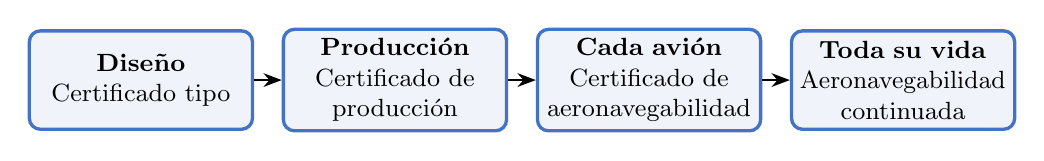
\begin{tikzpicture}[node distance=0.35cm, every node/.style={font=\small, align=center},
  paso/.style={draw=ppAzul, very thick, rounded corners, fill=ppAzul!8, text width=2.6cm,
  minimum height=1.25cm}]
  \node[paso] (a) {\textbf{Diseño}\\ Certificado tipo};
  \node[paso, right=of a] (b) {\textbf{Producción}\\ Certificado de producción};
  \node[paso, right=of b] (c) {\textbf{Cada avión}\\ Certificado de aeronavegabilidad};
  \node[paso, right=of c] (d) {\textbf{Toda su vida}\\ Aeronavegabilidad continuada};
  \draw[-{Stealth}, thick] (a) -- (b);
  \draw[-{Stealth}, thick] (b) -- (c);
  \draw[-{Stealth}, thick] (c) -- (d);
\end{tikzpicture}
\end{center}

\begin{center}
\small
\begin{tabular}{|p{0.27\linewidth}|p{0.18\linewidth}|p{0.45\linewidth}|}
\hline
\textbf{Documento} & \textbf{Quién lo obtiene} & \textbf{Qué certifica} \\ \hline
\textbf{Certificado tipo} (con su hoja de datos, \textbf{TCDS}) & El fabricante & Que el
\textbf{diseño} de un modelo de avión, motor o hélice cumple las normas de aeronavegabilidad
(RAAC 21 y 23/25/27/29). \\ \hline
\textbf{Certificado tipo suplementario} (STC) & Quien diseña una modificación & Que una
\textbf{modificación mayor} al diseño (por ejemplo, instalar una nueva aviónica integrada) es
aceptable. \\ \hline
\textbf{Certificado de producción} & El fabricante & Que puede fabricar en serie aeronaves o
partes iguales al diseño aprobado. \\ \hline
\textbf{Certificado de aeronavegabilidad} & Cada avión individual & Que \textbf{ese avión}
coincide con el diseño aprobado y está en condiciones de volar seguro. Sigue válido solo si se
mantiene según el programa de mantenimiento aprobado. Puede ser estándar o especial (restringido,
experimental, deportivo liviano, permiso especial de vuelo). \\ \hline
\textbf{Directiva de aeronavegabilidad} (AD) & La emite la autoridad & Una inspección o
modificación \textbf{obligatoria} ante un problema descubierto en servicio. \\ \hline
\textbf{Aprobación para el retorno al servicio} & La firma una persona u organización habilitada
& Que, después de un trabajo de mantenimiento, el avión quedó aeronavegable. Esa firma tiene
\textbf{responsabilidad legal}. \\ \hline
\end{tabular}
\end{center}

\subsubsection*{2.1. Aeronavegabilidad continuada}
Una vez en servicio, la aeronave debe seguir siendo aeronavegable. Eso se logra con:
\begin{itemize}
  \item el \textbf{programa de mantenimiento} aprobado (inspecciones por horas de vuelo, ciclos o
        calendario);
  \item el cumplimiento de las \textbf{directivas de aeronavegabilidad (AD)};
  \item la evaluación de los \textbf{boletines de servicio (SB)} del fabricante: son
        recomendaciones, salvo que una AD los haga obligatorios;
  \item el control de los \textbf{componentes de vida limitada} (que deben retirarse al cumplir
        un número de horas o ciclos);
  \item los \textbf{registros} de todo lo realizado.
\end{itemize}

\begin{recuadro}
\textbf{Caso: UPS 2976 (Louisville, EE.\,UU., 4 de noviembre de 2025).} Un MD-11F de carga
perdió el motor izquierdo junto con su pilón durante el despegue y se estrelló; murieron los 3
tripulantes y 11 personas en tierra. La investigación de la NTSB encontró fisuras por fatiga en
un componente del montaje del pilón, y que el fabricante había documentado en 2011 fallas
anteriores de esa pieza en una carta de servicio, sin considerarlas un riesgo para la seguridad
del vuelo. Después del accidente, la FAA emitió \textbf{directivas de aeronavegabilidad de
emergencia} que obligaron a inspeccionar todos los MD-11 y DC-10 antes de volver a volar.
\textbf{Para discutir:} ¿qué diferencia hay entre una recomendación del fabricante y una AD? ¿Qué
rol juegan el operador y su programa de mantenimiento?
\end{recuadro}

% ------------------------------------------------------------
\section*{3. EL MANTENIMIENTO SEGÚN LA RAAC PARTE 43}

La \textbf{RAAC 43} define qué es mantenimiento y cómo debe hacerse y registrarse.

\begin{center}
\small
\begin{tabular}{|p{0.26\linewidth}|p{0.64\linewidth}|}
\hline
\textbf{Término} & \textbf{Significado} \\ \hline
Mantenimiento & Inspección, revisión general (\textit{overhaul}), reparación, conservación y
reemplazo de partes. \\ \hline
Mantenimiento preventivo & Tareas menores y simples de conservación y reemplazo de pequeñas
partes estándar, que no requieren operaciones de montaje complejas. La regulación las enumera.
\\ \hline
Reparación / alteración \textbf{mayor} & Puede afectar de manera apreciable el peso, el
balance, la resistencia estructural, el funcionamiento de los motores, las características de
vuelo u otras cualidades de aeronavegabilidad, o no puede hacerse con prácticas elementales.
Requiere \textbf{datos aprobados} y un formulario específico. \\ \hline
Reparación / alteración \textbf{menor} & Toda la que no es mayor. \\ \hline
Reconstrucción & Restaurar un producto a la condición de ``nuevo'', con partes nuevas o
equivalentes. \\ \hline
Retorno al servicio & Declaración, firmada por persona habilitada, de que el producto quedó
aeronavegable. \\ \hline
\end{tabular}
\end{center}

\paragraph*{¿Quién puede hacer mantenimiento y aprobar el retorno al servicio?}
Según los alcances de cada uno: el titular de una \textbf{licencia} de mecánico con las
habilitaciones correspondientes (RAAC 65), un \textbf{Taller Aeronáutico de Reparación} (RAAC 145)
a través de su representante técnico, un \textbf{explotador} con su propia organización de
mantenimiento (RAAC 121 o 135) y el \textbf{fabricante} para sus productos.

\paragraph*{El registro del trabajo.}
Todo trabajo debe quedar registrado en los historiales de la aeronave, motor, hélice o componente,
con al menos: \textbf{descripción del trabajo} (o referencia a datos aceptables), \textbf{fecha},
\textbf{nombre, firma y número de licencia} de quien aprueba el retorno al servicio. Las
reparaciones y alteraciones mayores se documentan además en un formulario específico (equivalente
al formulario 337 de la FAA). \textbf{Si no está registrado, para la ley no se hizo.}

% ------------------------------------------------------------
\section*{4. LOS DOCUMENTOS DE LA AERONAVE}

\subsubsection*{4.1. Documentos a bordo}
\begin{itemize}
  \item \textbf{Certificado de matrícula} (Registro Nacional de Aeronaves). La matrícula argentina
        empieza con \textbf{LV} (o LQ para aeronaves del Estado).
  \item \textbf{Certificado de aeronavegabilidad} vigente.
  \item \textbf{Manual de vuelo} aprobado (AFM) con sus limitaciones.
  \item \textbf{Licencia de la estación de radio} de a bordo.
  \item \textbf{Libro de a bordo} o registro técnico de vuelo, donde se anotan los vuelos y las
        fallas observadas.
  \item \textbf{Licencias y certificados médicos} de la tripulación; seguro obligatorio.
\end{itemize}

\subsubsection*{4.2. Historiales y registros de mantenimiento}
Historial de la célula, de cada motor y de cada hélice; registro del cumplimiento de AD;
control de componentes de vida limitada; tarjetas de trabajo (\textit{task cards}); peso y
balanceo actualizado; lista de equipos instalados.

\subsubsection*{4.3. Manuales técnicos}
\begin{center}
\small
\begin{tabular}{|p{0.16\linewidth}|p{0.74\linewidth}|}
\hline
\textbf{Sigla} & \textbf{Manual} \\ \hline
AMM & \textit{Aircraft Maintenance Manual}: procedimientos de mantenimiento de la aeronave. \\
\hline
IPC / IPB & \textit{Illustrated Parts Catalog}: catálogo ilustrado de partes con sus números de
parte (P/N) e intercambiabilidad. \\ \hline
WDM & \textit{Wiring Diagram Manual}: diagramas de cableado; el manual más usado por el técnico
aviónico. \\ \hline
SRM & \textit{Structural Repair Manual}: reparaciones estructurales. \\ \hline
CMM & \textit{Component Maintenance Manual}: mantenimiento de un componente en taller (por
ejemplo, un transceptor VHF). \\ \hline
MPD & \textit{Maintenance Planning Document}: tareas e intervalos para armar el programa de
mantenimiento. \\ \hline
MEL / MMEL & Lista de equipo mínimo: qué equipos pueden estar inoperativos y en qué condiciones
se puede despachar el avión igual. \\ \hline
FIM / TSM & Manual de aislamiento de fallas: guía de diagnóstico a partir de un mensaje o
síntoma. \\ \hline
\end{tabular}
\end{center}
Los manuales deben estar en su \textbf{última revisión}: trabajar con una copia vieja o
impresa ``para tenerla a mano'' es una causa clásica de errores.

% ------------------------------------------------------------
\section*{5. LAS PARTES AERONÁUTICAS}

Una parte solo puede instalarse en una aeronave si es una \textbf{parte aprobada} y está
acompañada de su \textbf{documentación de aeronavegabilidad}, que garantiza su origen y su estado:
\begin{itemize}
  \item \textbf{Formulario FAA 8130-3} o \textbf{EASA Form 1}: certificado de liberación
        autorizada de una parte nueva o reparada.
  \item \textbf{Certificado de conformidad} del fabricante.
  \item Partes fabricadas bajo \textbf{TSO} (orden técnica estándar), \textbf{PMA} (aprobación de
        fabricación de partes) o \textbf{partes estándar} reconocidas (AN, MS, NAS).
\end{itemize}

\paragraph*{Estados de una parte.} \textit{Serviciable} (lista para instalar, con su etiqueta y
certificado), \textit{inservible} o \textit{reparable} (con etiqueta roja o amarilla, separada
físicamente), \textit{chatarra} (debe inutilizarse para que no vuelva al circuito).

\begin{recuadro}
\textbf{Partes no aprobadas sospechosas (SUP).} Son partes de origen dudoso: falsificadas,
recuperadas de aviones accidentados sin control, con documentación adulterada o fuera de vida
útil. Están entre los riesgos más graves del mantenimiento. Señales de alerta: precio muy bajo,
documentación incompleta o fotocopiada, marcas borradas, vendedor desconocido. Ante la duda,
\textbf{la parte no se instala} y se reporta a la autoridad.
\end{recuadro}

% ------------------------------------------------------------
\section*{6. LOS ESTÁNDARES DE LA DOCUMENTACIÓN}

\subsubsection*{6.1. ATA 100 / ATA iSpec 2200}
La \textbf{especificación ATA 100} (hoy integrada en la \textbf{ATA iSpec 2200}) organiza toda la
documentación técnica en \textbf{capítulos numerados} iguales para todos los fabricantes. Así, el
sistema de comunicaciones está en el capítulo 23 tanto en un Boeing como en un Airbus o un
Embraer. La referencia completa tiene tres pares de números: \textbf{capítulo -- sección -- tema}.
Por ejemplo, \texttt{23-11-00} es el sistema de HF dentro de Comunicaciones.

\begin{center}
\small
\begin{tabular}{|c|p{0.32\linewidth}||c|p{0.32\linewidth}|}
\hline
\textbf{Cap.} & \textbf{Sistema} & \textbf{Cap.} & \textbf{Sistema} \\ \hline
05 & Límites de tiempo, inspecciones & 31 & \textbf{Instrumentos indicadores y registradores} \\
\hline
12 & Servicio (carga de fluidos) & 32 & Tren de aterrizaje \\ \hline
20 & Prácticas estándar & 33 & \textbf{Luces} \\ \hline
21 & Aire acondicionado & 34 & \textbf{Navegación} \\ \hline
\textbf{22} & \textbf{Piloto automático} & 42 & \textbf{Aviónica modular integrada} \\ \hline
\textbf{23} & \textbf{Comunicaciones} & 44 & \textbf{Sistemas de cabina (entretenimiento)} \\
\hline
\textbf{24} & \textbf{Energía eléctrica} & 45 & \textbf{Sistema central de mantenimiento} \\ \hline
26 & Protección contra incendio & 46 & \textbf{Sistemas de información} \\ \hline
28 & Combustible & 49 & APU (unidad de potencia auxiliar) \\ \hline
30 & Protección contra hielo y lluvia & 71--80 & Motor \\ \hline
\end{tabular}
\end{center}

\subsubsection*{6.2. ATA 104}
La especificación \textbf{ATA 104} define cómo se estructura la \textbf{capacitación} del personal
de mantenimiento en niveles crecientes: desde la familiarización general con la aeronave hasta
el nivel de mantenimiento de línea y base, y la especialización en sistemas o componentes. Es la
base de los cursos de tipo que dan los fabricantes y los centros de instrucción.

\subsubsection*{6.3. Normas de partes y componentes: AN, MS, NAS, MIL}
\begin{center}
\small
\begin{tabular}{|p{0.13\linewidth}|p{0.36\linewidth}|p{0.40\linewidth}|}
\hline
\textbf{Norma} & \textbf{Origen} & \textbf{Ejemplos} \\ \hline
\textbf{AN} & \textit{Army--Navy}: normas militares conjuntas de EE.\,UU. (desde los años 40). &
Bulones AN3 a AN20, tuercas AN365, arandelas AN960. \\ \hline
\textbf{MS} & \textit{Military Standard}: reemplazó a muchas normas AN. & Remaches MS20470,
tornillos MS24693, terminales y empalmes de cableado. \\ \hline
\textbf{NAS} & \textit{National Aerospace Standard}: normas de la industria aeroespacial de EE.\,UU.
& Tornillos NAS1352, bulones de alta resistencia NAS6203. \\ \hline
\textbf{MIL} & \textit{Military Specifications} y estándares militares. & Cable MIL-W-22759,
conectores MIL-DTL-38999, bus de datos \textbf{MIL-STD-1553}. \\ \hline
\end{tabular}
\end{center}
Las normas fijan material, dimensiones, tolerancias, tratamientos y ensayos. Por eso un tornillo
aeronáutico \textbf{nunca se reemplaza ``por uno parecido''}, sino por el \textbf{número de parte
exacto} del catálogo ilustrado.

\begin{recuadro}
\textbf{Caso: British Airways 5390 (Reino Unido, 1990).} Al reemplazar el parabrisas del piloto
de un BAC 1-11, un supervisor eligió los tornillos ``a ojo'' en el depósito, sin consultar el
catálogo: 84 de los 90 tornillos eran apenas más finos que los especificados. En vuelo, la presión
de cabina arrancó el parabrisas y el comandante quedó parcialmente fuera de la cabina; la
tripulación logró aterrizar y no hubo víctimas fatales. El caso muestra el valor del número de
parte, del catálogo y de la verificación independiente.
\end{recuadro}

\subsubsection*{6.4. Otros estándares que usa un técnico aviónico}
\begin{itemize}
  \item \textbf{ARINC:} estándares de la industria para aviónica (por ejemplo, el bus de datos
        \textbf{ARINC 429} y los formatos de equipos y bandejas).
  \item \textbf{RTCA DO-160:} ensayos ambientales de equipos de a bordo (temperatura, vibración,
        interferencia electromagnética). \textbf{DO-178C} y \textbf{DO-254}: desarrollo de
        software y hardware de aviónica.
  \item \textbf{ISO 9001} (gestión de la calidad) y sus versiones aeroespaciales \textbf{AS/EN
        9100} (fabricantes), \textbf{AS9110} (organizaciones de mantenimiento) y \textbf{AS9120}
        (distribuidores). Se conectan con el sistema de calidad que exige la RAAC 145.
\end{itemize}

% ------------------------------------------------------------
\section*{7. CÓMO SE CONECTA TODO}
Cada trabajo de mantenimiento recorre la misma cadena:
\begin{enumerate}
  \item Un técnico \textbf{con licencia (RAAC 65)}
  \item trabaja en un \textbf{taller certificado (RAAC 145)},
  \item sigue el \textbf{manual del fabricante, organizado por capítulos ATA},
  \item usa \textbf{partes aprobadas, con su documentación} y que cumplen las normas AN, MS, NAS
        o MIL,
  \item registra el trabajo y \textbf{firma el retorno al servicio} (RAAC 43),
  \item y así el avión mantiene su \textbf{certificado de aeronavegabilidad}.
\end{enumerate}

% ------------------------------------------------------------
\section*{8. ACTIVIDADES DE LA UNIDAD}
\begin{enumerate}
  \item \textbf{Recorrido de certificación:} tomar un trabajo de aviónica (por ejemplo, reemplazar
        un receptor VOR) y seguir todo el recorrido: ubicar el capítulo ATA del sistema;
        verificar el número de parte del componente en el catálogo; revisar si hay directivas
        de aeronavegabilidad aplicables; completar el registro de mantenimiento; indicar quién
        puede firmar el retorno al servicio y con qué licencia.
  \item \textbf{Verificación de aeronavegabilidad simulada:} con un juego de documentos de una
        aeronave (reales o preparados por el docente), verificar documentos a bordo, vencimientos
        de inspecciones, cumplimiento de AD y componentes de vida limitada. Informar si la
        aeronave es aeronavegable y por qué.
  \item \textbf{¿Mayor o menor?} Clasificar una lista de trabajos (cambiar una lámpara, instalar un
        GPS con pantalla nueva en el panel, reparar un cable, reemplazar un transpondedor por otro
        del mismo P/N) en mantenimiento preventivo, alteración menor o mayor.
  \item \textbf{Tabla comparativa de estándares} ISO, AN, MS, NAS y MIL, con su aplicación en
        mantenimiento y documentación técnica, y un ejemplo de pieza del taller de la escuela.
  \item \textbf{Partes sospechosas:} con tres certificados de partes (uno correcto, uno incompleto,
        uno adulterado), decidir cuál se acepta y redactar el informe de rechazo.
\end{enumerate}
  % Unidad 2: aeronavegabilidad, certificación y documentación técnica
% ============================================================
% UNIDAD 3: LICENCIAS, REPRESENTANTE TÉCNICO Y OFICINA TÉCNICA
% ============================================================
\clearpage
\section*{UNIDAD 3: LICENCIAS DEL PERSONAL Y OFICINA TÉCNICA}
\subsection*{El mecánico, el representante técnico y su ámbito legal}

\begin{recuadro}
\textbf{Objetivo de la unidad:} conocer las licencias del personal de mantenimiento, en especial
la del técnico aviónico; sus requisitos, atribuciones, limitaciones y obligaciones; el rol del
\textbf{representante técnico} de un taller y las funciones de la \textbf{oficina técnica}.
\end{recuadro}

% ------------------------------------------------------------
\section*{1. LAS LICENCIAS DEL PERSONAL AERONÁUTICO}

El Código Aeronáutico establece que el personal aeronáutico necesita una \textbf{licencia o
certificado de idoneidad} expedido por la autoridad para ejercer sus funciones. Los requisitos
siguen el \textbf{Anexo 1} de la OACI. Para el personal que no es tripulante de vuelo, la norma
es la \textbf{RAAC Parte 65}, ``Personal aeronáutico, excepto miembros de la tripulación de
vuelo''.

\begin{center}
\small
\begin{tabular}{|p{0.15\linewidth}|p{0.75\linewidth}|}
\hline
\textbf{Subparte} & \textbf{Licencia o certificado} \\ \hline
D & \textbf{Licencia de Mecánico de Mantenimiento de Aeronave (MMA)}. \\ \hline
J & \textbf{Licencia de Mecánico de Equipos Radioeléctricos de Aeronaves (MERA)}: \textbf{la
licencia del técnico aviónico}. \\ \hline
K & Certificado de competencia de certificador aeronáutico. \\ \hline
L & Certificado de competencia de tareas especiales de mantenimiento. \\ \hline
Otras & Controlador de tránsito aéreo, despachante de aeronave, operador de estación
aeronáutica, jefe de aeródromo, entre otras. \\ \hline
\end{tabular}
\end{center}

% ------------------------------------------------------------
\section*{2. LA LICENCIA MERA}

\subsubsection*{2.1. Requisitos para obtenerla por primera vez}
Con la Resolución ANAC N° 443/2025 se actualizaron los requisitos de las licencias MMA y MERA.
Para la licencia MERA se pide, en síntesis:
\begin{itemize}
  \item Tener \textbf{18 años}.
  \item Ser capaz de hablar, leer, escribir y entender el idioma español.
  \item Acreditar estudios (certificado de nivel primario o secundario).
  \item Poseer el \textbf{título} de Mecánico de Equipos Radioeléctricos de Aeronave o de
        Mecánico de Aviónica otorgado por un Centro de Instrucción certificado bajo la RAAC 147,
        \textbf{o el título de Técnico en Aviónica (o equivalente) emitido por una escuela
        técnica}.
  \item Un \textbf{certificado médico aeronáutico} vigente, de la clase que exija la regulación
        (RAAC Parte 67).
  \item La inscripción vigente en el \textbf{Consejo Profesional de la Ingeniería Aeronáutica y
        Espacial (CPIAyE)}.
  \item DNI, formulario de solicitud, foto y el pago del arancel.
\end{itemize}
El trámite se inicia por la plataforma de \textbf{Trámites a Distancia (TAD)} o en forma
presencial con turno. La autoridad puede verificar el cumplimiento de los requisitos y tomar los
exámenes que correspondan.

\subsubsection*{2.2. Habilitaciones y recategorización}
La licencia se completa con \textbf{habilitaciones}, que indican qué trabajos puede certificar su
titular (en la MMA, categorías A, B o C; en la MERA, la habilitación en aviónica). Para obtenerlas
hay que \textbf{acreditar experiencia de trabajo} con un formulario específico, además de los
requisitos generales.

\subsubsection*{2.3. Atribuciones y limitaciones}
\begin{itemize}
  \item El titular de una licencia \textbf{sin habilitación} puede realizar tareas de
        mantenimiento, pero \textbf{bajo la supervisión} de un titular habilitado con atribuciones
        para esas tareas.
  \item Con la habilitación correspondiente puede realizar y \textbf{certificar} los trabajos
        incluidos en ella, y firmar los registros de mantenimiento dentro de sus atribuciones.
  \item Nunca puede certificar trabajos fuera de las atribuciones de su licencia y habilitación,
        ni sobre tipos de equipos o aeronaves para los que no tiene la instrucción y la experiencia
        necesarias.
\end{itemize}

\subsubsection*{2.4. Validez y obligaciones del titular}
\begin{itemize}
  \item Mantener vigente el \textbf{certificado médico} y no ejercer cuando su aptitud física o
        mental esté disminuida (enfermedad, medicamentos, fatiga).
  \item \textbf{No trabajar bajo los efectos del alcohol o de drogas.}
  \item Llevar consigo la licencia y exhibirla cuando la autoridad lo requiera.
  \item Trabajar con la documentación técnica vigente y las herramientas adecuadas y calibradas.
  \item \textbf{Registrar con veracidad} todo trabajo realizado. Falsear un registro es una falta
        gravísima.
  \item Mantenerse actualizado (cursos, nuevos equipos, cambios normativos).
\end{itemize}

\begin{recuadro}
\textbf{Responsabilidad legal.} Cuando un técnico firma un retorno al servicio, asume la
responsabilidad de que el trabajo se hizo bien y de que la aeronave o el componente quedó
aeronavegable. Si no lo hizo correctamente, puede sufrir \textbf{sanciones administrativas}
(apercibimiento, suspensión o inhabilitación de la licencia por parte de la ANAC) y, si hay daños,
\textbf{responsabilidad civil} (indemnizar) y \textbf{penal} (por ejemplo, por estrago u homicidio
culposo). La firma no es un trámite: es una garantía personal.
\end{recuadro}

% ------------------------------------------------------------
\section*{3. EL REPRESENTANTE TÉCNICO}

\subsubsection*{3.1. Definición}
La RAAC 145 define al \textbf{representante técnico (RT)} como la persona designada por el Taller
Aeronáutico de Reparación (TAR) que:
\begin{itemize}
  \item es \textbf{responsable del retorno al servicio} de cualquier artículo procesado por el
        taller;
  \item asume la \textbf{responsabilidad técnica sobre todas las operaciones} del taller que se
        realizan según la RAAC 145, incluido asegurar que el personal cumpla las regulaciones; y
  \item \textbf{representa al taller ante la autoridad aeronáutica} (ANAC).
\end{itemize}
Junto a él existe el \textbf{gerente responsable}, que tiene la autoridad corporativa (y los
recursos económicos) para asegurar que todo el mantenimiento pueda hacerse según las
regulaciones. Para certificar un taller, la ANAC pide los antecedentes del representante técnico
propuesto y una nota en la que acepta el cargo.

\subsubsection*{3.2. Funciones, derechos y obligaciones}
\begin{center}
\small
\begin{tabular}{|p{0.44\linewidth}|p{0.46\linewidth}|}
\hline
\textbf{Funciones y obligaciones} & \textbf{Derechos y facultades} \\ \hline
\begin{itemize}[leftmargin=*,nosep]
  \item Firmar los retornos al servicio (o designar a quienes lo hagan según el manual).
  \item Mantener actualizado el manual del taller y la lista de capacidades.
  \item Controlar que el personal tenga licencias, habilitaciones e instrucción.
  \item Asegurar herramientas calibradas, documentación vigente e instalaciones adecuadas.
  \item Comunicar a la ANAC cambios, fallas y defectos graves.
  \item Atender las inspecciones y auditorías de la autoridad.
\end{itemize}
&
\begin{itemize}[leftmargin=*,nosep]
  \item Detener un trabajo o negarse a firmar un retorno al servicio si no está conforme, aunque
        lo presione el cliente o la empresa.
  \item Exigir a la empresa los recursos necesarios para trabajar según la norma.
  \item Rechazar partes sin documentación válida.
  \item Ser consultado ante cualquier cambio que afecte la operación técnica del taller.
\end{itemize}
\\ \hline
\end{tabular}
\end{center}

\subsubsection*{3.3. Organigrama funcional de un taller}
\begin{center}
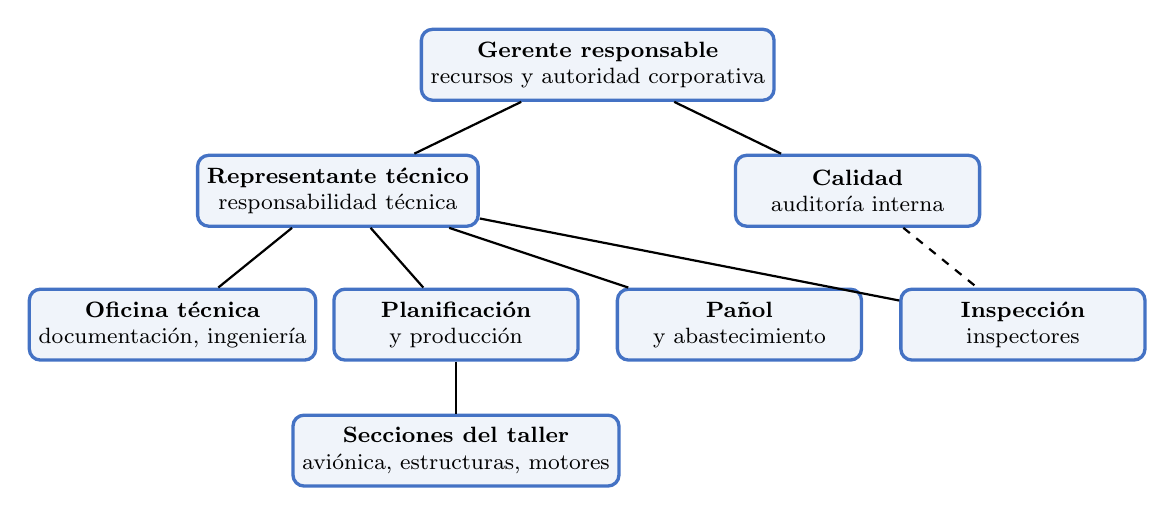
\begin{tikzpicture}[every node/.style={font=\footnotesize, align=center},
  caja/.style={draw=ppAzul, very thick, rounded corners, fill=ppAzul!8, minimum width=3.1cm,
  minimum height=0.9cm}]
  \node[caja] (g) at (0,0) {\textbf{Gerente responsable}\\ recursos y autoridad corporativa};
  \node[caja] (rt) at (-3.3,-1.6) {\textbf{Representante técnico}\\ responsabilidad técnica};
  \node[caja] (cal) at (3.3,-1.6) {\textbf{Calidad}\\ auditoría interna};
  \node[caja] (ot) at (-5.4,-3.3) {\textbf{Oficina técnica}\\ documentación, ingeniería};
  \node[caja] (pl) at (-1.8,-3.3) {\textbf{Planificación}\\ y producción};
  \node[caja] (pa) at (1.8,-3.3) {\textbf{Pañol}\\ y abastecimiento};
  \node[caja] (in) at (5.4,-3.3) {\textbf{Inspección}\\ inspectores};
  \node[caja] (sec) at (-1.8,-4.9) {\textbf{Secciones del taller}\\ aviónica, estructuras, motores};
  \draw[thick] (g) -- (rt); \draw[thick] (g) -- (cal);
  \draw[thick] (rt) -- (ot); \draw[thick] (rt) -- (pl); \draw[thick] (rt) -- (pa);
  \draw[thick] (rt) -- (in); \draw[thick] (pl) -- (sec);
  \draw[thick, dashed] (cal) -- (in);
\end{tikzpicture}
\end{center}
La función de \textbf{calidad} debe ser \textbf{independiente} de la producción: quien inspecciona
no debe depender de quien tiene que terminar el trabajo a tiempo.

% ------------------------------------------------------------
\section*{4. LA OFICINA TÉCNICA}

La \textbf{oficina técnica} es el ``cerebro documental'' de un taller o de un operador. Es uno de
los ámbitos de trabajo más importantes para un técnico con experiencia.

\subsubsection*{4.1. Funciones}
\begin{itemize}
  \item \textbf{Biblioteca técnica:} recibir, controlar y distribuir los manuales en su última
        revisión; retirar las revisiones viejas.
  \item \textbf{Ingeniería:} evaluar las directivas de aeronavegabilidad y los boletines de
        servicio que aplican a cada aeronave; estudiar modificaciones; obtener los
        \textbf{datos aprobados} para reparaciones y alteraciones mayores.
  \item \textbf{Planificación:} armar las órdenes de trabajo y las tarjetas de tareas a partir del
        programa de mantenimiento.
  \item \textbf{Registros:} mantener los historiales de aeronaves, motores y componentes, y el
        control de vencimientos y vidas límite.
  \item \textbf{Relación con la autoridad:} preparar las presentaciones, formularios e informes, y
        atender las inspecciones.
\end{itemize}

\subsubsection*{4.2. Planos, memorias y documentación técnica}
\begin{itemize}
  \item \textbf{Planos:} de conjunto, de detalle, de instalación y \textbf{diagramas eléctricos}
        (esquemáticos, de cableado y de conexionado). Hay que saber leer las vistas, las cotas,
        las tolerancias, los símbolos y la \textbf{lista de materiales}.
  \item \textbf{Memoria técnica:} documento que describe y justifica un trabajo de ingeniería. Para
        una instalación de aviónica suele incluir: descripción del equipo y de la modificación,
        normas aplicables, ubicación y fijación, diagrama eléctrico, \textbf{análisis de carga
        eléctrica} (que el sistema de generación soporte el nuevo consumo), cálculo de \textbf{peso
        y balanceo}, compatibilidad electromagnética, ensayos funcionales y suplemento al manual
        de vuelo si corresponde.
  \item \textbf{Órdenes de trabajo y tarjetas de tareas}, con los pasos, las herramientas, los
        valores de prueba y las firmas de quien ejecuta y de quien inspecciona.
\end{itemize}

\subsubsection*{4.3. La relación con la autoridad de aeronavegabilidad}
Históricamente, la aeronavegabilidad estaba a cargo de la \textbf{Dirección Nacional de
Aeronavegabilidad (DNA)}; hoy esas funciones están en la \textbf{ANAC}, dentro de su Dirección
Nacional de Seguridad Operacional. La oficina técnica se relaciona con ella para:
\begin{itemize}
  \item presentar los trabajos de reparación y alteración mayor y sus datos;
  \item solicitar aprobaciones, inspecciones de aeronavegabilidad y certificados;
  \item informar fallas, defectos y dificultades en servicio;
  \item responder a las observaciones de las auditorías.
\end{itemize}

% ------------------------------------------------------------
\section*{5. ACTIVIDADES DE LA UNIDAD}
\begin{enumerate}
  \item \textbf{Simulación de emisión de la licencia MERA:} armar la carpeta completa de
        solicitud con todos los requisitos (formulario, documentación, título, certificado médico,
        inscripción profesional, pago). Un grupo actúa como ``autoridad'' y la revisa: ¿está
        completa?, ¿qué falta?
  \item \textbf{Atribuciones:} para cinco situaciones del taller, decidir si un técnico con
        licencia sin habilitación, uno con habilitación o el representante técnico puede hacer y
        firmar el trabajo.
  \item \textbf{Organigrama funcional} de un TAR de aviónica, con las funciones, derechos y
        obligaciones del representante técnico.
  \item \textbf{Memoria técnica:} redactar la memoria de la instalación de un transpondedor con
        ADS-B en un avión liviano, incluyendo diagrama eléctrico y análisis de carga eléctrica.
  \item \textbf{Registro y retorno al servicio:} completar el registro de un trabajo de aviónica
        con todos sus datos y la firma de retorno al servicio.
  \item \textbf{Dilema ético:} el cliente apura la entrega de un avión y falta una prueba
        funcional. ¿Qué hace el representante técnico? ¿Qué dice la norma? ¿Qué riesgos hay?
\end{enumerate}
      % Unidad 3: licencias, representante técnico y oficina técnica
% ============================================================
% UNIDAD 4: ORGANIZACIONES AERONÁUTICAS Y GESTIÓN DEL MANTENIMIENTO
% ============================================================
\clearpage
\section*{UNIDAD 4: ORGANIZACIONES AERONÁUTICAS}
\subsection*{Gestión, producción, servicios y economía del mantenimiento}

\begin{recuadro}
\textbf{Objetivo de la unidad:} comprender cómo se organizan las empresas del sector aeronáutico,
cómo se planifica y controla el mantenimiento, cómo se abastecen y comercializan partes y
servicios, qué indicadores se usan para gestionar y cuánto pesa el mantenimiento en la economía
de un operador, sin dejar de lado la calidad, el ambiente y la salud laboral.
\end{recuadro}

% ------------------------------------------------------------
\section*{1. LAS ORGANIZACIONES DEL SECTOR}

\begin{center}
\small
\begin{tabular}{|p{0.27\linewidth}|p{0.14\linewidth}|p{0.47\linewidth}|}
\hline
\textbf{Organización} & \textbf{Norma} & \textbf{Qué hace} \\ \hline
Fabricantes de aeronaves, motores, equipos y partes & RAAC 21 & Diseñan y producen bajo
certificado tipo y de producción. \\ \hline
Explotadores aerocomerciales & RAAC 119, 121, 135 & Transportan pasajeros y carga (líneas
aéreas, taxis aéreos). \\ \hline
Explotadores de trabajo aéreo & RAAC 137 & Aviación agrícola, fotografía, inspección. \\ \hline
Aviación general & RAAC 91 & Aeroclubes, propietarios privados, aviación corporativa. \\ \hline
\textbf{Talleres Aeronáuticos de Reparación (TAR)} & \textbf{RAAC 145} & Mantienen, reparan y
modifican aeronaves y componentes para terceros. \\ \hline
Centros de instrucción & RAAC 141, 142, 147 & Forman pilotos y mecánicos. \\ \hline
Proveedores de servicios de navegación aérea & -- & Control de tránsito, radioayudas, radares
(EANA). \\ \hline
Aeropuertos & RAAC 153 & Infraestructura y servicios en tierra. \\ \hline
Distribuidores de partes & -- & Venden y certifican partes y componentes. \\ \hline
\end{tabular}
\end{center}

\subsubsection*{1.1. La estructura de un operador aéreo}
Un explotador aerocomercial tiene, como mínimo, áreas de \textbf{Operaciones} (vuelos y
tripulaciones), \textbf{Mantenimiento e Ingeniería}, \textbf{Calidad}, \textbf{Seguridad
operacional (SMS)}, \textbf{Comercial}, \textbf{Administración y Finanzas} y \textbf{Recursos
Humanos}. Para cada área clave la autoridad exige un \textbf{responsable designado} con la
calificación adecuada.

Dentro de Mantenimiento conviene distinguir dos funciones: la \textbf{gestión de la
aeronavegabilidad continuada} (decidir qué hay que hacer y cuándo: programa, AD, confiabilidad,
registros) y la \textbf{ejecución del mantenimiento} (hacerlo), que puede hacer el propio operador
o contratar a un TAR.

% ------------------------------------------------------------
\section*{2. PRODUCCIÓN Y SERVICIOS: EL MANTENIMIENTO}

\subsubsection*{2.1. Mantenimiento de línea y de base}
\begin{itemize}
  \item \textbf{De línea:} se hace entre vuelos, en la plataforma: inspecciones de tránsito y
        diarias, solución de fallas reportadas por la tripulación, cambio rápido de componentes
        (LRU, \textit{Line Replaceable Unit}). Ahí trabaja mucho el técnico aviónico.
  \item \textbf{De base o pesado:} se hace en hangar, con el avión fuera de servicio varios días
        o semanas: inspecciones mayores, reparaciones estructurales, modificaciones.
\end{itemize}

\subsubsection*{2.2. El programa de mantenimiento}
Las tareas se programan por intervalos de \textbf{horas de vuelo (FH)}, \textbf{ciclos (FC:
despegue y aterrizaje)} o \textbf{calendario}, lo que ocurra primero. En los aviones de línea se
agrupan en \textbf{chequeos}: los más frecuentes y livianos (``A'') y los más espaciados y
profundos (``C'' y, en algunos programas, ``D''). Los programas modernos se elaboran con la
metodología \textbf{MSG-3}, que analiza las consecuencias de cada falla para decidir qué tarea
conviene y con qué frecuencia.

Los componentes se gestionan con tres criterios:
\begin{itemize}
  \item \textbf{Tiempo límite (\textit{hard time}):} se retiran al cumplir su vida, estén como
        estén.
  \item \textbf{A condición (\textit{on condition}):} se inspeccionan o ensayan periódicamente y
        se retiran si no pasan la prueba.
  \item \textbf{Monitoreo de condición:} se usan hasta que fallan, controlando estadísticamente su
        confiabilidad. Es típico de muchos equipos de aviónica, cuya falla es detectable y no
        compromete la seguridad (hay redundancia).
\end{itemize}

\subsubsection*{2.3. Planificación y programación}
La planificación convierte el programa en trabajo concreto: prevé qué aviones vencen qué tareas,
reserva lugar en el hangar, calcula las \textbf{horas-hombre} necesarias, arma el \textbf{paquete
de trabajo} con sus órdenes y tarjetas, y anticipa partes, herramientas y personal licenciado. Una
buena planificación reduce el tiempo en tierra y evita trabajos apurados (y errores).

% ------------------------------------------------------------
\section*{3. ABASTECIMIENTO Y COMERCIALIZACIÓN}

\subsubsection*{3.1. Selección y abastecimiento de partes}
\begin{itemize}
  \item \textbf{Proveedores aprobados:} el taller u operador mantiene una lista de proveedores
        evaluados (calidad, documentación, plazos). Comprar fuera de ella exige una evaluación
        especial.
  \item \textbf{Tipos de partes:} \textbf{rotables} (componentes reparables con número de serie que
        rotan entre avión y taller, como un transceptor o una computadora), \textbf{reparables} y
        \textbf{consumibles} (que se usan una vez: juntas, filtros, tornillería).
  \item \textbf{Intercambio (\textit{exchange}):} se recibe un componente serviciable y se entrega
        el averiado para su reparación, pagando la reparación más una diferencia. Reduce el
        tiempo de avión en tierra.
  \item \textbf{Inspección de recepción:} verificar número de parte, número de serie, estado y
        documentación (8130-3, EASA Form 1) antes de ingresar la parte al pañol.
  \item \textbf{Stock:} definir mínimos y puntos de pedido según consumo y criticidad; las piezas
        que pueden dejar un avión en tierra se priorizan.
\end{itemize}

\subsubsection*{3.2. Comercialización de servicios y equipos}
Un taller vende capacidad técnica: debe tener claro su \textbf{alcance} (lista de capacidades
aprobada por la ANAC), sus \textbf{tiempos de entrega} (TAT, \textit{turn around time}), sus
\textbf{precios} (horas-hombre más materiales), las \textbf{garantías} que ofrece y los
\textbf{contratos} que firma. En aviónica, además, es común la representación y venta de equipos de
fabricantes extranjeros con su instalación y soporte.

% ------------------------------------------------------------
\section*{4. CONTROL DE GESTIÓN}

El \textbf{control de gestión} compara lo planificado con lo real usando \textbf{indicadores}
(KPI), para detectar desvíos y corregirlos a tiempo.

\begin{center}
\small
\begin{tabular}{|p{0.15\linewidth}|p{0.42\linewidth}|p{0.31\linewidth}|}
\hline
\textbf{Área} & \textbf{Indicador} & \textbf{Qué muestra} \\ \hline
Técnica & \textbf{Confiabilidad de despacho}: \% de salidas sin demora técnica & Si el
mantenimiento cumple su objetivo. \\ \hline
Técnica & \textbf{MTBF} (tiempo medio entre fallas) y \textbf{MTBUR} (entre remociones no
programadas) & Confiabilidad de cada componente; detecta equipos ``problemáticos''. \\ \hline
Técnica & Fallas repetitivas, eventos AOG, reportes de pilotos & Calidad del diagnóstico y
de las reparaciones. \\ \hline
Económica & Costo de mantenimiento por hora de vuelo; presupuesto vs.\ real; valor del stock &
Eficiencia y control del gasto. \\ \hline
Comercial & TAT, cumplimiento de plazos, reclamos, facturación & Satisfacción del cliente. \\
\hline
Personal & Horas-hombre productivas, horas extra, capacitación, ausentismo, rotación &
Cargas de trabajo y fatiga (que se conectan con la seguridad). \\ \hline
\end{tabular}
\end{center}

% ------------------------------------------------------------
\section*{5. LA ECONOMÍA DEL OPERADOR Y EL MANTENIMIENTO}

Para un operador, el \textbf{combustible} suele ser el mayor costo, y el \textbf{mantenimiento}
está entre los principales, junto con el personal y el costo de los aviones (compra o
\textit{leasing}). Pero el mantenimiento también influye en los \textbf{ingresos}: un avión en
tierra no vende pasajes.

\begin{recuadro}
\textbf{Caso práctico (valores hipotéticos).} Un operador regional vuela cada avión
\textbf{2.500 horas por año}. Sus costos anuales de mantenimiento por avión son:
\begin{center}
\begin{tabular}{|p{0.55\linewidth}|r|}
\hline
Mantenimiento de línea (personal, materiales) & USD 300.000 \\ \hline
Chequeos de base (prorrateados por año) & USD 400.000 \\ \hline
Reserva para revisiones de motores (USD 250/h $\times$ 2 motores $\times$ 2.500 h) &
USD 1.250.000 \\ \hline
Componentes y reparaciones (USD 150/h $\times$ 2.500 h) & USD 375.000 \\ \hline
\textbf{Total anual por avión} & \textbf{USD 2.325.000} \\ \hline
\textbf{Costo de mantenimiento por hora de vuelo} & \textbf{USD 930} \\ \hline
\end{tabular}
\end{center}
\textbf{Costo de un día AOG:} si el avión hace 6 vuelos por día con 60 pasajeros y un pasaje
medio de USD 100, un día en tierra significa perder unos \textbf{USD 36.000} de ingresos, más la
reubicación de pasajeros y el impacto en la imagen. Por eso conviene invertir en stock de
componentes críticos, en buena planificación y en técnicos bien capacitados.
\end{recuadro}

% ------------------------------------------------------------
\section*{6. CALIDAD, AMBIENTE Y SALUD LABORAL}

\subsubsection*{6.1. Gestión de la calidad}
La RAAC 145 exige un \textbf{sistema de control de calidad} descripto en el manual del taller:
inspección de recepción, inspección durante y después del trabajo, control de herramientas y
calibraciones, auditorías internas, acciones correctivas. Muchos talleres además se certifican en
\textbf{ISO 9001} o \textbf{AS9110}. Calidad y seguridad operacional se complementan: la calidad
verifica que se cumplan los procedimientos; el SMS gestiona los riesgos (Unidad 6).

\subsubsection*{6.2. Protección ambiental}
\begin{itemize}
  \item \textbf{Residuos peligrosos} (Ley 24.051 y normas provinciales): aceites, combustibles,
        fluidos hidráulicos, solventes, pinturas, baterías y residuos electrónicos deben separarse,
        almacenarse rotulados y entregarse a transportistas y operadores habilitados.
  \item \textbf{Derrames:} bateas, materiales absorbentes y procedimientos de respuesta.
  \item \textbf{Ruido y emisiones:} el Anexo 16 de la OACI fija límites para aeronaves y
        motores.
  \item La norma \textbf{ISO 14001} ofrece un sistema de gestión ambiental certificable.
\end{itemize}

\subsubsection*{6.3. Salud y seguridad en el trabajo}
El marco general es la \textbf{Ley 19.587} de Higiene y Seguridad en el Trabajo y la \textbf{Ley
24.557} de Riesgos del Trabajo (ART). Riesgos típicos de un hangar y de un taller de aviónica:
\begin{center}
\small
\begin{tabular}{|p{0.32\linewidth}|p{0.58\linewidth}|}
\hline
\textbf{Riesgo} & \textbf{Prevención} \\ \hline
Caídas en altura (alas, empenaje) & Plataformas con baranda, arnés, escaleras en buen estado. \\
\hline
Ruido de motores y APU & Protección auditiva, zonas delimitadas. \\ \hline
Electricidad (115 V 400 Hz, 28 V DC, fuentes de tierra) & Bloqueo y etiquetado de
interruptores, verificación de ausencia de tensión. \\ \hline
\textbf{Radiofrecuencia}: radar meteorológico y transmisores & No operar el radar en tierra con
personas o combustible cerca del cono de emisión; respetar distancias del manual. \\ \hline
Químicos (fluidos hidráulicos, solventes, combustible) & Guantes, anteojos, ventilación, hojas de
seguridad. \\ \hline
Descarga electrostática (ESD) & Pulsera y superficies antiestáticas al manipular equipos
sensibles. \\ \hline
Objetos extraños (FOD) & Control de herramientas y limpieza de plataforma. \\ \hline
\end{tabular}
\end{center}

% ------------------------------------------------------------
\section*{7. ACTIVIDADES DE LA UNIDAD}
\begin{enumerate}
  \item \textbf{Plan de mantenimiento:} para una flota simulada de tres aviones con sus horas, ciclos
        y vencimientos, armar el plan anual de chequeos y detectar superposiciones.
  \item \textbf{Control de gestión:} con datos de un año de operación (salidas, demoras, remociones
        de componentes), calcular la confiabilidad de despacho y el MTBUR de dos equipos de
        aviónica, y proponer acciones.
  \item \textbf{Economía del operador:} con el caso práctico, calcular cómo cambia el costo por
        hora si el avión vuela 2.000 o 3.000 horas por año, y cuántos días AOG ``paga'' tener un
        transceptor de repuesto en stock.
  \item \textbf{Esquema de gestión de un emprendimiento aeronáutico:} diseñar la organización de un
        pequeño taller de aviónica (producción, previsión de servicios, abastecimiento y
        comercialización de equipos), con su organigrama, sus indicadores y su lista de
        capacidades.
  \item \textbf{Relevamiento de riesgos laborales y ambientales} del taller de la escuela, con
        propuestas de mejora.
\end{enumerate}
 % Unidad 4: organizaciones aeronáuticas y gestión del mantenimiento
% ============================================================
% UNIDAD 5: ACTUACIÓN HUMANA
% ============================================================
\clearpage
\section*{UNIDAD 5: ACTUACIÓN HUMANA}
\subsection*{Factores humanos, error, MRM, reportes y primeros auxilios}

\begin{recuadro}
\textbf{Objetivo de la unidad:} reconocer que el desempeño humano es un factor crítico en el
mantenimiento aeronáutico, identificar los factores que lo afectan, entender cómo se producen los
errores y aplicar herramientas para prevenirlos, reportarlos e investigarlos (MRM y MEDA).
Incluye una práctica de primeros auxilios adaptada al entorno del hangar.
\end{recuadro}

% ------------------------------------------------------------
\section*{1. POR QUÉ IMPORTAN LOS FACTORES HUMANOS}

Los aviones modernos son muy confiables, pero los opera, controla y mantiene gente. En la gran
mayoría de los accidentes e incidentes aparece, entre las causas, algún \textbf{factor humano}:
una decisión, una omisión, una mala comunicación, una presión de la organización. El estudio de
los \textbf{factores humanos} busca entender cómo trabajan las personas para diseñar tareas,
equipos, procedimientos y organizaciones que \textbf{reduzcan la posibilidad de error y atrapen
los errores antes de que causen daño}.

\paragraph*{El modelo SHELL.}
Representa a la persona (\textbf{L}, \textit{Liveware}) en el centro, en relación con:
\begin{center}
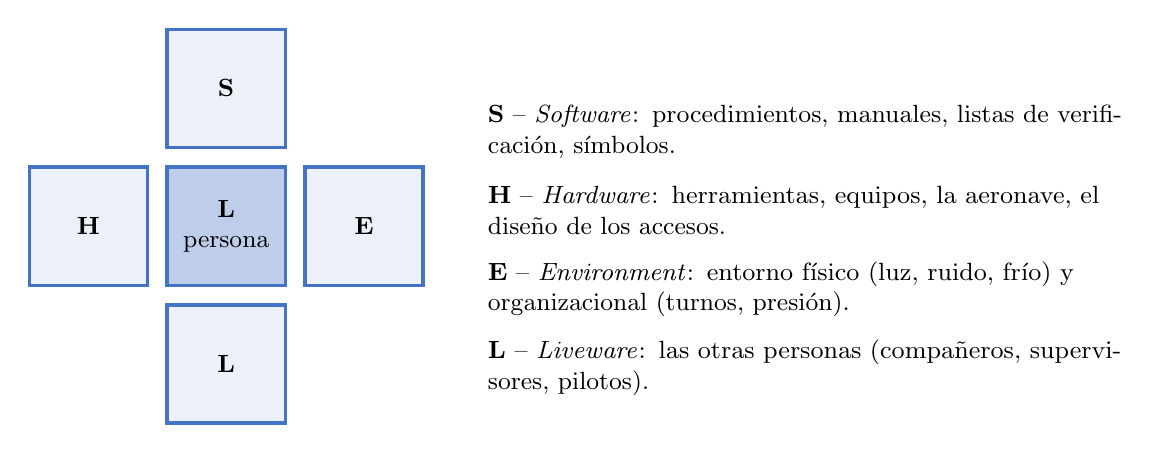
\begin{tikzpicture}[every node/.style={font=\small, align=center},
  b/.style={draw=ppAzul, very thick, fill=ppAzul!10, minimum width=1.5cm, minimum height=1.5cm}]
  \node[b, fill=ppAzul!35] (L) at (0,0) {\textbf{L}\\ persona};
  \node[b] (S) at (0,1.75) {\textbf{S}};
  \node[b] (H) at (-1.75,0) {\textbf{H}};
  \node[b] (E) at (1.75,0) {\textbf{E}};
  \node[b] (L2) at (0,-1.75) {\textbf{L}};
  \node[anchor=west, text width=8cm, align=left] at (3.2,1.2) {\textbf{S} -- \textit{Software}:
  procedimientos, manuales, listas de verificación, símbolos.};
  \node[anchor=west, text width=8cm, align=left] at (3.2,0.2) {\textbf{H} -- \textit{Hardware}:
  herramientas, equipos, la aeronave, el diseño de los accesos.};
  \node[anchor=west, text width=8cm, align=left] at (3.2,-0.8) {\textbf{E} -- \textit{Environment}:
  entorno físico (luz, ruido, frío) y organizacional (turnos, presión).};
  \node[anchor=west, text width=8cm, align=left] at (3.2,-1.8) {\textbf{L} -- \textit{Liveware}:
  las otras personas (compañeros, supervisores, pilotos).};
\end{tikzpicture}
\end{center}
Los errores suelen aparecer en las \textbf{interfaces}, donde ``no encajan'' la persona y lo
demás: un manual confuso (L--S), un conector al que no se llega (L--H), un hangar oscuro (L--E),
un pase de turno mal hecho (L--L).

% ------------------------------------------------------------
\section*{2. FACTORES QUE AFECTAN EL RENDIMIENTO}

\begin{center}
\small
\begin{tabular}{|p{0.22\linewidth}|p{0.68\linewidth}|}
\hline
\textbf{Tipo} & \textbf{Ejemplos} \\ \hline
Físicos & Visión (agudeza, colores: clave para identificar cables), audición, fuerza, tamaño
corporal. \\ \hline
Fisiológicos & \textbf{Fatiga} y falta de sueño, trabajo nocturno (ritmo circadiano), hambre,
deshidratación, enfermedad, \textbf{alcohol, drogas y medicamentos}. \\ \hline
Psicológicos & Estrés, atención y distracción, memoria, percepción, motivación, exceso de
confianza o \textbf{complacencia}. \\ \hline
Entorno físico & Iluminación, ruido, temperatura, clima, espacio de trabajo reducido, trabajo en
altura. \\ \hline
Organización del trabajo & Turnos largos, presión de tiempo, falta de personal o de repuestos,
procedimientos inadecuados, cultura de la empresa. \\ \hline
\end{tabular}
\end{center}

\begin{recuadro}
\textbf{La fatiga se parece al alcohol.} Estudios clásicos mostraron que estar despierto unas
17 horas seguidas deteriora el desempeño de manera comparable a tener 0,5 gramos de alcohol por
litro de sangre, y estar despierto 24 horas, a 1 g/l. Nadie trabajaría ``borracho'' en un avión;
sin embargo, trabajar sin dormir es frecuente. Por eso las organizaciones gestionan las horas de
trabajo y descanso, y cada técnico debe reconocer cuándo no está en condiciones.
\end{recuadro}

% ------------------------------------------------------------
\section*{3. LA DOCENA SUCIA}

Gordon Dupont, de Transport Canada, identificó doce condiciones que más a menudo llevan a errores
de mantenimiento. Se conocen como la \textbf{docena sucia} (\textit{Dirty Dozen}):

\begin{center}
\small
\begin{tabular}{|c|p{0.27\linewidth}|p{0.57\linewidth}|}
\hline
\textbf{N°} & \textbf{Factor} & \textbf{Defensa} \\ \hline
1 & Falta de comunicación & Pase de turno por escrito; confirmar lo entendido. \\ \hline
2 & Complacencia & Verificar siempre como si fuera la primera vez. \\ \hline
3 & Falta de conocimiento & Capacitación; consultar el manual; preguntar. \\ \hline
4 & Distracción & Marcar dónde quedó el trabajo; volver tres pasos atrás al retomarlo. \\ \hline
5 & Falta de trabajo en equipo & Planificar juntos; compartir información. \\ \hline
6 & Fatiga & Descansar; reconocer los síntomas; pedir doble control. \\ \hline
7 & Falta de recursos & Pedir las herramientas y partes correctas; no improvisar. \\ \hline
8 & Presión & Comunicar si no se llega; ``mejor tarde que nunca''. \\ \hline
9 & Falta de asertividad & Decir lo que se piensa, con respeto y con datos. \\ \hline
10 & Estrés & Pausas; tomar las cosas de a una; pedir ayuda. \\ \hline
11 & Falta de conciencia situacional & Pensar qué puede pasar después; preguntarse ``¿y si...?''. \\
\hline
12 & Normas informales (``siempre se hizo así'') & Seguir el procedimiento aprobado; si está mal,
cambiarlo formalmente. \\ \hline
\end{tabular}
\end{center}

% ------------------------------------------------------------
\section*{4. EL ERROR HUMANO}

El psicólogo \textbf{James Reason} distinguió entre:
\begin{itemize}
  \item \textbf{Errores} (no intencionales):
  \begin{itemize}
    \item \textbf{Deslices:} la intención era correcta pero la acción salió mal (girar la llave
          equivocada).
    \item \textbf{Lapsus:} olvidos (no colocar un tornillo, no cerrar una tapa).
    \item \textbf{Equivocaciones:} el plan estaba mal (diagnóstico equivocado por falta de
          conocimiento).
  \end{itemize}
  \item \textbf{Violaciones} (desvíos intencionales de un procedimiento):
  \begin{itemize}
    \item \textbf{Rutinarias:} ``todos lo hacen así'' (no usar el torquímetro).
    \item \textbf{Situacionales:} para cumplir con un plazo o por falta de recursos.
    \item \textbf{Excepcionales:} en situaciones fuera de lo común.
  \end{itemize}
\end{itemize}
\textbf{Errores típicos en mantenimiento:} instalaciones incompletas, partes mal instaladas o
equivocadas, herramientas o materiales olvidados dentro de la aeronave, conectores sin trabar,
falta de verificación funcional, registros incompletos y \textbf{errores en el pase de turno}.

\paragraph*{La idea clave.} Los errores no se pueden eliminar del todo: las personas se equivocan.
Lo que sí se puede hacer es \textbf{reducir las condiciones que los provocan}, \textbf{detectarlos}
(inspecciones, verificaciones) y \textbf{limitar sus consecuencias} (redundancia, defensas).

% ------------------------------------------------------------
\section*{5. TRABAJO EN EQUIPO, COMUNICACIÓN Y MRM}

\subsubsection*{5.1. Del CRM al MRM}
Después de accidentes como Tenerife (1977), en los que la comunicación y el liderazgo en la
cabina fallaron, la industria desarrolló el \textbf{CRM} (\textit{Crew Resource Management}):
entrenamiento de las tripulaciones en comunicación, liderazgo, toma de decisiones y uso de todos
los recursos disponibles. En los años noventa, tras accidentes causados por errores de
mantenimiento, se adaptó a los talleres como \textbf{MRM} (\textit{Maintenance Resource
Management}).

\subsubsection*{5.2. Contenidos de un programa de MRM}
\begin{itemize}
  \item \textbf{Comunicación:} clara, completa, confirmada (``lectura y colación''); por escrito en
        los pases de turno.
  \item \textbf{Asertividad:} expresar una preocupación de seguridad aunque el otro tenga más
        jerarquía. Una fórmula útil: llamar la atención (``Jefe...''), plantear el problema (``veo
        que...''), proponer una acción (``propongo que...'') y pedir una respuesta (``¿de
        acuerdo?'').
  \item \textbf{Trabajo en equipo y liderazgo}, planificación de tareas compartidas.
  \item \textbf{Conciencia situacional:} saber qué está pasando, qué falta y qué puede pasar.
  \item \textbf{Toma de decisiones} y manejo del estrés y la fatiga.
  \item \textbf{Docena sucia} y cultura de reporte.
\end{itemize}

% ------------------------------------------------------------
\section*{6. SELECCIÓN E INSTRUCCIÓN DEL PERSONAL}
\begin{itemize}
  \item \textbf{Selección:} definir el perfil del puesto (licencias, habilitaciones, experiencia,
        idioma técnico inglés) y evaluar también actitudes: responsabilidad, trabajo en equipo,
        atención al detalle.
  \item \textbf{Instrucción inicial:} sistema de calidad, procedimientos del taller, factores
        humanos, seguridad laboral.
  \item \textbf{Instrucción en el puesto} (OJT): bajo supervisión, con registro de las tareas
        aprendidas.
  \item \textbf{Cursos de tipo} de aeronaves o equipos (ATA 104).
  \item \textbf{Instrucción recurrente}: actualización periódica en normas, factores humanos y
        cambios técnicos.
  \item Registro de toda la instrucción, porque la autoridad lo audita.
\end{itemize}

% ------------------------------------------------------------
\section*{7. PREVENCIÓN DE ERRORES EN EL TALLER}
\begin{itemize}
  \item \textbf{Procedimientos y tarjetas de tareas} claros, con pasos verificables.
  \item \textbf{Listas de verificación} (\textit{checklists}) para las tareas críticas.
  \item \textbf{Inspección independiente} (doble inspección) de las tareas que, mal hechas, pueden
        causar una falla catastrófica: controles de vuelo, fijación de motores.
  \item \textbf{Control de herramientas}: tableros de sombra y conteo al terminar.
  \item \textbf{Señalización de trabajos incompletos} y \textbf{pase de turno} por escrito.
  \item \textbf{Manejo de las interrupciones}: marcar el punto, y al retomar volver unos pasos atrás.
  \item \textbf{Gestión de la fatiga}: límites de horas, descansos, rotación de tareas.
\end{itemize}

% ------------------------------------------------------------
\section*{8. REPORTES E INVESTIGACIÓN DE ERRORES}

\subsubsection*{8.1. La cultura justa}
Si cada error se castiga, la gente lo esconde, y la organización pierde la oportunidad de
aprender. Una \textbf{cultura justa} (\textit{just culture}) alienta a reportar errores y
peligros \textbf{sin temor a sanciones}, pero deja claro que no se toleran las conductas
temerarias, las violaciones deliberadas ni el consumo de alcohol o drogas. El límite está entre
el \textbf{error honesto} (se aprende de él) y la \textbf{negligencia grave} (se sanciona).

\subsubsection*{8.2. Tipos de reportes}
\begin{itemize}
  \item \textbf{Obligatorios:} los sucesos que la norma exige notificar a la autoridad o a la JST
        (accidentes, incidentes graves, ciertas fallas).
  \item \textbf{Voluntarios:} errores, peligros o ``casi accidentes'' que cualquiera puede informar,
        muchas veces en forma confidencial.
\end{itemize}

\subsubsection*{8.3. El método MEDA}
El \textbf{MEDA} (\textit{Maintenance Error Decision Aid}), desarrollado por Boeing, es una
herramienta para investigar los errores de mantenimiento buscando \textbf{por qué} ocurrieron, no
\textbf{quién} tuvo la culpa. Se basa en la idea de que el técnico no quiere equivocarse: el error
aparece por \textbf{factores contribuyentes} que la organización puede corregir.

\begin{center}
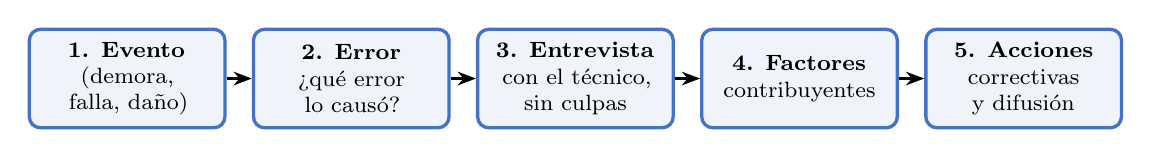
\begin{tikzpicture}[node distance=0.32cm, every node/.style={font=\footnotesize, align=center},
  paso/.style={draw=ppAzul, very thick, rounded corners, fill=ppAzul!8, text width=2.25cm,
  minimum height=1.25cm}]
  \node[paso] (a) {\textbf{1. Evento}\\ (demora, falla, daño)};
  \node[paso, right=of a] (b) {\textbf{2. Error}\\ ¿qué error lo causó?};
  \node[paso, right=of b] (c) {\textbf{3. Entrevista}\\ con el técnico, sin culpas};
  \node[paso, right=of c] (d) {\textbf{4. Factores}\\ contribuyentes};
  \node[paso, right=of d] (e) {\textbf{5. Acciones}\\ correctivas y difusión};
  \draw[-{Stealth}, thick] (a) -- (b); \draw[-{Stealth}, thick] (b) -- (c);
  \draw[-{Stealth}, thick] (c) -- (d); \draw[-{Stealth}, thick] (d) -- (e);
\end{tikzpicture}
\end{center}
Los factores contribuyentes se buscan en categorías: información (manuales, tarjetas), equipos y
herramientas, diseño y configuración de la aeronave, tarea, conocimientos y habilidades, factores
individuales (fatiga, presión), entorno, organización, liderazgo y supervisión, comunicación.

% ------------------------------------------------------------
\section*{9. MONITOREO Y AUDITORÍA}
La organización verifica que sus defensas funcionan mediante \textbf{auditorías internas}
(documentales y en el puesto de trabajo), \textbf{observación de tareas} por pares entrenados,
seguimiento de \textbf{indicadores} (errores reportados, fallas repetitivas, retrabajos) y
verificación de que las acciones correctivas se cumplieron y fueron eficaces.

% ------------------------------------------------------------
\section*{10. PRIMEROS AUXILIOS EN EL ENTORNO DE MANTENIMIENTO}

\begin{recuadro}
\textbf{Importante:} esta sección es una introducción. La práctica de RCP y uso del DEA debe
hacerse con un instructor capacitado y con muñecos de entrenamiento. Ante una emergencia, llamar
siempre a los servicios de emergencia (\textbf{107} o \textbf{911}) y al servicio médico de la
empresa o del aeropuerto.
\end{recuadro}

\paragraph*{La regla PAS.} \textbf{P}roteger (asegurar la escena: cortar la energía, alejar del
peligro, no convertirse en otra víctima), \textbf{A}visar (llamar a emergencias, dar ubicación
exacta), \textbf{S}ocorrer (asistir a la víctima).

\begin{center}
\small
\begin{tabular}{|p{0.22\linewidth}|p{0.68\linewidth}|}
\hline
\textbf{Situación} & \textbf{Qué hacer} \\ \hline
Persona que no responde y no respira normalmente & Llamar a emergencias, pedir un
\textbf{DEA} (desfibrilador) y empezar la \textbf{RCP}: compresiones fuertes y rápidas en el centro
del pecho, de 100 a 120 por minuto, sin interrupciones, hasta que llegue el DEA o la ayuda. \\
\hline
\textbf{Electrocución} & No tocar a la víctima hasta \textbf{cortar la energía} (fuente de tierra,
baterías, interruptor). Luego evaluar y actuar. \\ \hline
Hemorragia & Presión directa y firme sobre la herida con un apósito o tela limpia. \\ \hline
Quemadura térmica & Enfriar con agua corriente durante varios minutos; no aplicar cremas ni
hielo; no despegar la ropa adherida. \\ \hline
Contacto con químicos (fluidos hidráulicos, combustible) & Lavar con abundante agua; en los ojos,
lavado prolongado. Consultar la hoja de seguridad del producto. \\ \hline
Caída de altura & No mover a la víctima (posible lesión de columna), salvo peligro inminente. \\
\hline
\end{tabular}
\end{center}

% ------------------------------------------------------------
\section*{11. ACTIVIDADES DE LA UNIDAD}
\begin{enumerate}
  \item \textbf{SHELL:} analizar una tarea del taller de la escuela con el modelo SHELL e
        identificar una interfaz problemática en cada letra.
  \item \textbf{Docena sucia en el taller:} durante una semana, cada estudiante registra situaciones
        propias en las que apareció alguno de los doce factores y qué defensa podría haber usado.
  \item \textbf{Simulación de pase de turno (MRM):} ver la actividad práctica a continuación.
  \item \textbf{Investigación MEDA:} a partir de un error simulado (por ejemplo, un conector sin
        trabar detectado en la prueba funcional), entrevistar al ``técnico'', completar la planilla
        de factores contribuyentes y proponer acciones.
  \item \textbf{Primeros auxilios:} práctica de RCP con muñeco y simulación de rescate de un
        electrocutado en el taller, con un instructor.
\end{enumerate}
       % Unidad 5: actuación humana, MRM y primeros auxilios
% ============================================================
% ACTIVIDAD PRÁCTICA: SIMULACIÓN DE PASE DE TURNO (MRM)
% Se puede usar sola o con % ============================================================
% ACTIVIDAD PRÁCTICA: SIMULACIÓN DE PASE DE TURNO (MRM)
% Se puede usar sola o con % ============================================================
% ACTIVIDAD PRÁCTICA: SIMULACIÓN DE PASE DE TURNO (MRM)
% Se puede usar sola o con \input{actividad_mrm} dentro del manual.
% ============================================================
\clearpage
\section*{ACTIVIDAD PRÁCTICA: SIMULACIÓN DE PASE DE TURNO}
\subsection*{Factores humanos en mantenimiento (MRM)}

\begin{recuadro}
\textbf{Objetivo:} experimentar cómo una mala comunicación en el pase de turno genera errores
de mantenimiento, identificar los factores humanos que intervienen (la ``docena sucia'') y
aplicar una herramienta concreta del MRM, la planilla de pase de turno, para prevenirlos.
\end{recuadro}

\paragraph*{Duración:} 2 módulos (80 a 120 minutos).
\paragraph*{Lugar:} taller o laboratorio de aviónica.
\paragraph*{Materiales:}
\begin{itemize}
  \item Un equipo o panel por grupo, con tapas atornilladas y conectores desmontables
        (por ejemplo, una caja de instrumentos de práctica, una fuente o un equipo en desuso).
  \item Herramientas de mano y un recipiente para tornillería.
  \item Cinta o tarjetas de ``trabajo incompleto'' para señalizar.
  \item Copias de la \textbf{Planilla de pase de turno} y de la \textbf{Planilla de registro}
        (al final de esta actividad).
  \item Cronómetro.
\end{itemize}

% ------------------------------------------------------------
\subsubsection*{1. Introducción (15 minutos)}
El docente presenta brevemente los dos casos reales y la docena sucia.

\paragraph*{Continental Express 2574 (Texas, EE.\,UU., 1991).}
Durante el turno noche se comenzó a cambiar los bordes de ataque del estabilizador
horizontal de un Embraer 120. Se retiraron los tornillos superiores de uno de los lados,
pero el trabajo quedó sin terminar. El aviso en el pase de turno fue verbal y no llegó a
quien continuaba la tarea. El avión salió con esa pieza sujeta solo por los tornillos
inferiores; se desprendió en vuelo y murieron los 14 ocupantes.

\paragraph*{British Airways 5390 (Reino Unido, 1990).}
De noche y con poco personal, un supervisor reemplazó el parabrisas del piloto de un
BAC 1-11 eligiendo los tornillos ``a ojo'', sin consultar el catálogo de partes. La mayoría
eran levemente más finos que los especificados. En vuelo, la presión de cabina arrancó el
parabrisas; el comandante quedó parcialmente fuera del avión y fue sostenido por la
tripulación hasta el aterrizaje.

\begin{center}
\small
\textbf{La ``docena sucia'' (\textit{Dirty Dozen}) de factores humanos en mantenimiento}\\[3pt]
\begin{tabular}{|p{0.29\linewidth}|p{0.29\linewidth}|p{0.29\linewidth}|}
\hline
1. Falta de comunicación & 5. Falta de trabajo en equipo & 9. Falta de asertividad \\ \hline
2. Complacencia & 6. Fatiga & 10. Estrés \\ \hline
3. Falta de conocimiento & 7. Falta de recursos & 11. Falta de conciencia situacional \\ \hline
4. Distracción & 8. Presión & 12. Normas (malas costumbres del grupo) \\ \hline
\end{tabular}
\end{center}

% ------------------------------------------------------------
\subsubsection*{2. Organización}
El curso se divide en grupos de 4 a 6 integrantes. Cada grupo trabaja sobre su propio
equipo y se divide en dos ``turnos'':
\begin{itemize}
  \item \textbf{Turno A (saliente):} comienza el trabajo y lo deja a medias.
  \item \textbf{Turno B (entrante):} recibe el trabajo y debe terminarlo.
  \item \textbf{Un observador} por grupo (puede rotar): no participa del trabajo, registra lo
        que ocurre en la Planilla de registro.
\end{itemize}
El docente entrega al Turno A una \textbf{orden de trabajo} escrita, que el Turno B
\textbf{no ve}. Ejemplo de orden de trabajo:
\begin{enumerate}
  \item Retirar la tapa superior del equipo.
  \item Desconectar los conectores J1 y J3.
  \item Retirar el módulo interno indicado por el docente.
  \item Volver a instalar el módulo, reconectar J1 y J3 y colocar la tapa con todos sus
        tornillos.
  \item Verificar el funcionamiento.
\end{enumerate}

% ------------------------------------------------------------
\subsubsection*{3. Ronda 1: pase de turno ``informal'' (20 minutos)}
\begin{enumerate}
  \item El Turno A realiza los pasos 1 a 3 y, antes de terminar, el docente anuncia el
        \textbf{fin del turno}. El docente puede agregar, sin avisar, alguna condición extra
        (por ejemplo, dejar un tornillo de la tapa colocado sin ajustar).
  \item El Turno A tiene \textbf{un minuto} para contarle al Turno B, \textbf{solo de palabra},
        en qué quedó el trabajo. No pueden escribir ni mostrar el equipo.
  \item El Turno B termina el trabajo, \textbf{sin ver la orden de trabajo} y sin hacer
        preguntas al Turno A.
  \item El observador registra todo en la Planilla de registro.
\end{enumerate}

% ------------------------------------------------------------
\subsubsection*{4. Ronda 2: pase de turno con planilla (25 minutos)}
Se repite el ejercicio sobre el mismo equipo (o se intercambian los equipos entre grupos), y
\textbf{se invierten los roles}: quienes fueron Turno B ahora son Turno A. Esta vez:
\begin{enumerate}
  \item El Turno A completa la \textbf{Planilla de pase de turno} antes de irse y
        \textbf{señaliza} en el equipo lo que quedó abierto o desconectado.
  \item El pase se hace \textbf{cara a cara, frente al equipo}, leyendo la planilla. El Turno B
        puede hacer preguntas y firma que recibió el trabajo.
  \item El Turno B termina la tarea usando la planilla y la orden de trabajo, y realiza una
        \textbf{verificación final} antes de cerrar.
  \item El observador vuelve a completar la Planilla de registro.
\end{enumerate}

% ------------------------------------------------------------
\subsubsection*{5. Puesta en común (20 minutos)}
Cada grupo compara los resultados de las dos rondas y responde:
\begin{enumerate}
  \item ¿Cuántos errores u omisiones hubo en cada ronda? (tornillos faltantes o flojos,
        conectores sin reconectar o cruzados, pasos omitidos, verificación no realizada).
  \item ¿Qué factores de la docena sucia aparecieron en la Ronda 1? Den un ejemplo concreto de
        cada uno.
  \item ¿Qué cambió en la Ronda 2? ¿Qué parte de la planilla fue la más útil?
  \item ¿Alguien del Turno B notó que algo no cerraba y no lo dijo? ¿Por qué? (asertividad,
        presión de tiempo).
  \item ¿Qué tienen en común sus errores con los casos de Continental Express 2574 y
        British Airways 5390?
  \item Propongan una mejora para la planilla de pase de turno del taller de la escuela.
\end{enumerate}

% ------------------------------------------------------------
\subsubsection*{6. Evaluación}
\begin{itemize}
  \item Participación y cumplimiento del rol asignado en ambas rondas.
  \item Calidad y claridad de la Planilla de pase de turno completada.
  \item Correcta identificación de los factores humanos en la puesta en común.
  \item Respuestas escritas a las preguntas del punto 5 (entrega individual o grupal).
\end{itemize}

\begin{recuadro}
\textbf{Idea central:} en mantenimiento, \textbf{lo que no está escrito no está hecho}. El
pase de turno se hace por escrito, cara a cara y frente al trabajo; ante la duda se verifica
con la documentación aprobada y nunca se supone.
\end{recuadro}

% ============================================================
% PLANILLA DE PASE DE TURNO (para imprimir)
% ============================================================
\clearpage
\begin{center}
{\large\bfseries PLANILLA DE PASE DE TURNO}\\[2pt]
{\small Taller de Aviónica -- E.E.S.T. N° 7 ``Taller Regional Quilmes''}
\end{center}

\renewcommand{\arraystretch}{1.4}
\noindent
\begin{tabular}{|>{\raggedright\arraybackslash}p{0.34\linewidth}|p{0.595\linewidth}|}
\hline
\textbf{Fecha} & \\ \hline
\textbf{Equipo / aeronave} & \\ \hline
\textbf{N° de orden de trabajo} & \\ \hline
\textbf{Turno saliente (nombres)} & \\ \hline
\textbf{Turno entrante (nombres)} & \\ \hline
\end{tabular}

\vspace{5pt}
\noindent\textbf{1. Tareas realizadas} (con el paso de la orden de trabajo)\\[2pt]
\begin{tabular}{|p{0.10\linewidth}|p{0.60\linewidth}|p{0.215\linewidth}|}
\hline
\textbf{Paso} & \textbf{Descripción de lo realizado} & \textbf{Firma} \\ \hline
 & & \\ \hline
 & & \\ \hline
 & & \\ \hline
\end{tabular}

\vspace{5pt}
\noindent\textbf{2. Tareas pendientes}\\[2pt]
\begin{tabular}{|p{0.10\linewidth}|p{0.83\linewidth}|}
\hline
\textbf{Paso} & \textbf{Qué falta hacer} \\ \hline
 & \\ \hline
 & \\ \hline
 & \\ \hline
\end{tabular}

\vspace{5pt}
\noindent\textbf{3. Estado en que queda el equipo}\\[2pt]
\begin{tabular}{|p{0.45\linewidth}|p{0.48\linewidth}|}
\hline
\textbf{Desmontado / desconectado} & \textbf{Dónde quedó (ubicación, rótulo)} \\ \hline
 & \\ \hline
 & \\ \hline
\textbf{Tornillería / fijaciones retiradas} & \textbf{Cantidad y dónde están} \\ \hline
 & \\ \hline
\end{tabular}

\vspace{5pt}
\noindent
\begin{tabular}{|p{0.62\linewidth}|c|c|}
\hline
\textbf{4. Verificaciones} & \textbf{Sí} & \textbf{No} \\ \hline
¿Se señalizó en el equipo que el trabajo está incompleto? & \hspace{0.6cm} & \hspace{0.6cm} \\ \hline
¿Hay herramientas o elementos sueltos dentro del equipo? & & \\ \hline
¿Se informó alguna anomalía o duda? (detallar abajo) & & \\ \hline
\end{tabular}

\vspace{5pt}
\noindent\textbf{5. Observaciones, anomalías o advertencias}\\[2pt]
\begin{tabular}{|p{0.955\linewidth}|}
\hline
\\ \hline
\\ \hline
\end{tabular}

\vspace{10pt}
\noindent
\begin{tabular}{|p{0.46\linewidth}|p{0.46\linewidth}|}
\hline
\textbf{Entrega (turno saliente)} & \textbf{Recibe (turno entrante)} \\
Firma y aclaración: & Firma y aclaración: \\[14pt] \hline
\end{tabular}
\renewcommand{\arraystretch}{1.15}

% ============================================================
% PLANILLA DE REGISTRO DEL OBSERVADOR (para imprimir)
% ============================================================
\clearpage
\begin{center}
{\large\bfseries PLANILLA DE REGISTRO DEL OBSERVADOR}\\[2pt]
{\small Simulación de pase de turno -- MRM}
\end{center}

\renewcommand{\arraystretch}{1.6}
\noindent
\begin{tabular}{|>{\raggedright\arraybackslash}p{0.34\linewidth}|p{0.595\linewidth}|}
\hline
\textbf{Grupo} & \\ \hline
\textbf{Observador/a} & \\ \hline
\end{tabular}

\vspace{8pt}
\noindent\textbf{Errores y omisiones detectados}\\[2pt]
\begin{tabular}{|p{0.50\linewidth}|>{\centering\arraybackslash}p{0.19\linewidth}|>{\centering\arraybackslash}p{0.19\linewidth}|}
\hline
\textbf{Tipo de error} & \textbf{Ronda 1} & \textbf{Ronda 2} \\ \hline
Tornillos faltantes, flojos o sobrantes & & \\ \hline
Conectores sin reconectar o cruzados & & \\ \hline
Pasos de la orden de trabajo omitidos & & \\ \hline
Componente mal instalado & & \\ \hline
Herramienta o elemento olvidado en el equipo & & \\ \hline
Verificación final no realizada & & \\ \hline
\textbf{Total} & & \\ \hline
\end{tabular}

\vspace{8pt}
\noindent\textbf{Factores de la docena sucia observados} (marcar y anotar un ejemplo)\\[2pt]
\begin{tabular}{|p{0.36\linewidth}|>{\centering\arraybackslash}p{0.08\linewidth}|>{\centering\arraybackslash}p{0.08\linewidth}|p{0.34\linewidth}|}
\hline
\textbf{Factor} & \textbf{R1} & \textbf{R2} & \textbf{Ejemplo observado} \\ \hline
1. Falta de comunicación & & & \\ \hline
2. Complacencia & & & \\ \hline
3. Falta de conocimiento & & & \\ \hline
4. Distracción & & & \\ \hline
5. Falta de trabajo en equipo & & & \\ \hline
6. Fatiga & & & \\ \hline
7. Falta de recursos & & & \\ \hline
8. Presión & & & \\ \hline
9. Falta de asertividad & & & \\ \hline
10. Estrés & & & \\ \hline
11. Falta de conciencia situacional & & & \\ \hline
12. Normas & & & \\ \hline
\end{tabular}

\vspace{8pt}
\noindent\textbf{Comentarios del observador}\\[2pt]
\begin{tabular}{|p{0.955\linewidth}|}
\hline
\\ \hline
\\ \hline
\\ \hline
\end{tabular}
\renewcommand{\arraystretch}{1.15}
 dentro del manual.
% ============================================================
\clearpage
\section*{ACTIVIDAD PRÁCTICA: SIMULACIÓN DE PASE DE TURNO}
\subsection*{Factores humanos en mantenimiento (MRM)}

\begin{recuadro}
\textbf{Objetivo:} experimentar cómo una mala comunicación en el pase de turno genera errores
de mantenimiento, identificar los factores humanos que intervienen (la ``docena sucia'') y
aplicar una herramienta concreta del MRM, la planilla de pase de turno, para prevenirlos.
\end{recuadro}

\paragraph*{Duración:} 2 módulos (80 a 120 minutos).
\paragraph*{Lugar:} taller o laboratorio de aviónica.
\paragraph*{Materiales:}
\begin{itemize}
  \item Un equipo o panel por grupo, con tapas atornilladas y conectores desmontables
        (por ejemplo, una caja de instrumentos de práctica, una fuente o un equipo en desuso).
  \item Herramientas de mano y un recipiente para tornillería.
  \item Cinta o tarjetas de ``trabajo incompleto'' para señalizar.
  \item Copias de la \textbf{Planilla de pase de turno} y de la \textbf{Planilla de registro}
        (al final de esta actividad).
  \item Cronómetro.
\end{itemize}

% ------------------------------------------------------------
\subsubsection*{1. Introducción (15 minutos)}
El docente presenta brevemente los dos casos reales y la docena sucia.

\paragraph*{Continental Express 2574 (Texas, EE.\,UU., 1991).}
Durante el turno noche se comenzó a cambiar los bordes de ataque del estabilizador
horizontal de un Embraer 120. Se retiraron los tornillos superiores de uno de los lados,
pero el trabajo quedó sin terminar. El aviso en el pase de turno fue verbal y no llegó a
quien continuaba la tarea. El avión salió con esa pieza sujeta solo por los tornillos
inferiores; se desprendió en vuelo y murieron los 14 ocupantes.

\paragraph*{British Airways 5390 (Reino Unido, 1990).}
De noche y con poco personal, un supervisor reemplazó el parabrisas del piloto de un
BAC 1-11 eligiendo los tornillos ``a ojo'', sin consultar el catálogo de partes. La mayoría
eran levemente más finos que los especificados. En vuelo, la presión de cabina arrancó el
parabrisas; el comandante quedó parcialmente fuera del avión y fue sostenido por la
tripulación hasta el aterrizaje.

\begin{center}
\small
\textbf{La ``docena sucia'' (\textit{Dirty Dozen}) de factores humanos en mantenimiento}\\[3pt]
\begin{tabular}{|p{0.29\linewidth}|p{0.29\linewidth}|p{0.29\linewidth}|}
\hline
1. Falta de comunicación & 5. Falta de trabajo en equipo & 9. Falta de asertividad \\ \hline
2. Complacencia & 6. Fatiga & 10. Estrés \\ \hline
3. Falta de conocimiento & 7. Falta de recursos & 11. Falta de conciencia situacional \\ \hline
4. Distracción & 8. Presión & 12. Normas (malas costumbres del grupo) \\ \hline
\end{tabular}
\end{center}

% ------------------------------------------------------------
\subsubsection*{2. Organización}
El curso se divide en grupos de 4 a 6 integrantes. Cada grupo trabaja sobre su propio
equipo y se divide en dos ``turnos'':
\begin{itemize}
  \item \textbf{Turno A (saliente):} comienza el trabajo y lo deja a medias.
  \item \textbf{Turno B (entrante):} recibe el trabajo y debe terminarlo.
  \item \textbf{Un observador} por grupo (puede rotar): no participa del trabajo, registra lo
        que ocurre en la Planilla de registro.
\end{itemize}
El docente entrega al Turno A una \textbf{orden de trabajo} escrita, que el Turno B
\textbf{no ve}. Ejemplo de orden de trabajo:
\begin{enumerate}
  \item Retirar la tapa superior del equipo.
  \item Desconectar los conectores J1 y J3.
  \item Retirar el módulo interno indicado por el docente.
  \item Volver a instalar el módulo, reconectar J1 y J3 y colocar la tapa con todos sus
        tornillos.
  \item Verificar el funcionamiento.
\end{enumerate}

% ------------------------------------------------------------
\subsubsection*{3. Ronda 1: pase de turno ``informal'' (20 minutos)}
\begin{enumerate}
  \item El Turno A realiza los pasos 1 a 3 y, antes de terminar, el docente anuncia el
        \textbf{fin del turno}. El docente puede agregar, sin avisar, alguna condición extra
        (por ejemplo, dejar un tornillo de la tapa colocado sin ajustar).
  \item El Turno A tiene \textbf{un minuto} para contarle al Turno B, \textbf{solo de palabra},
        en qué quedó el trabajo. No pueden escribir ni mostrar el equipo.
  \item El Turno B termina el trabajo, \textbf{sin ver la orden de trabajo} y sin hacer
        preguntas al Turno A.
  \item El observador registra todo en la Planilla de registro.
\end{enumerate}

% ------------------------------------------------------------
\subsubsection*{4. Ronda 2: pase de turno con planilla (25 minutos)}
Se repite el ejercicio sobre el mismo equipo (o se intercambian los equipos entre grupos), y
\textbf{se invierten los roles}: quienes fueron Turno B ahora son Turno A. Esta vez:
\begin{enumerate}
  \item El Turno A completa la \textbf{Planilla de pase de turno} antes de irse y
        \textbf{señaliza} en el equipo lo que quedó abierto o desconectado.
  \item El pase se hace \textbf{cara a cara, frente al equipo}, leyendo la planilla. El Turno B
        puede hacer preguntas y firma que recibió el trabajo.
  \item El Turno B termina la tarea usando la planilla y la orden de trabajo, y realiza una
        \textbf{verificación final} antes de cerrar.
  \item El observador vuelve a completar la Planilla de registro.
\end{enumerate}

% ------------------------------------------------------------
\subsubsection*{5. Puesta en común (20 minutos)}
Cada grupo compara los resultados de las dos rondas y responde:
\begin{enumerate}
  \item ¿Cuántos errores u omisiones hubo en cada ronda? (tornillos faltantes o flojos,
        conectores sin reconectar o cruzados, pasos omitidos, verificación no realizada).
  \item ¿Qué factores de la docena sucia aparecieron en la Ronda 1? Den un ejemplo concreto de
        cada uno.
  \item ¿Qué cambió en la Ronda 2? ¿Qué parte de la planilla fue la más útil?
  \item ¿Alguien del Turno B notó que algo no cerraba y no lo dijo? ¿Por qué? (asertividad,
        presión de tiempo).
  \item ¿Qué tienen en común sus errores con los casos de Continental Express 2574 y
        British Airways 5390?
  \item Propongan una mejora para la planilla de pase de turno del taller de la escuela.
\end{enumerate}

% ------------------------------------------------------------
\subsubsection*{6. Evaluación}
\begin{itemize}
  \item Participación y cumplimiento del rol asignado en ambas rondas.
  \item Calidad y claridad de la Planilla de pase de turno completada.
  \item Correcta identificación de los factores humanos en la puesta en común.
  \item Respuestas escritas a las preguntas del punto 5 (entrega individual o grupal).
\end{itemize}

\begin{recuadro}
\textbf{Idea central:} en mantenimiento, \textbf{lo que no está escrito no está hecho}. El
pase de turno se hace por escrito, cara a cara y frente al trabajo; ante la duda se verifica
con la documentación aprobada y nunca se supone.
\end{recuadro}

% ============================================================
% PLANILLA DE PASE DE TURNO (para imprimir)
% ============================================================
\clearpage
\begin{center}
{\large\bfseries PLANILLA DE PASE DE TURNO}\\[2pt]
{\small Taller de Aviónica -- E.E.S.T. N° 7 ``Taller Regional Quilmes''}
\end{center}

\renewcommand{\arraystretch}{1.4}
\noindent
\begin{tabular}{|>{\raggedright\arraybackslash}p{0.34\linewidth}|p{0.595\linewidth}|}
\hline
\textbf{Fecha} & \\ \hline
\textbf{Equipo / aeronave} & \\ \hline
\textbf{N° de orden de trabajo} & \\ \hline
\textbf{Turno saliente (nombres)} & \\ \hline
\textbf{Turno entrante (nombres)} & \\ \hline
\end{tabular}

\vspace{5pt}
\noindent\textbf{1. Tareas realizadas} (con el paso de la orden de trabajo)\\[2pt]
\begin{tabular}{|p{0.10\linewidth}|p{0.60\linewidth}|p{0.215\linewidth}|}
\hline
\textbf{Paso} & \textbf{Descripción de lo realizado} & \textbf{Firma} \\ \hline
 & & \\ \hline
 & & \\ \hline
 & & \\ \hline
\end{tabular}

\vspace{5pt}
\noindent\textbf{2. Tareas pendientes}\\[2pt]
\begin{tabular}{|p{0.10\linewidth}|p{0.83\linewidth}|}
\hline
\textbf{Paso} & \textbf{Qué falta hacer} \\ \hline
 & \\ \hline
 & \\ \hline
 & \\ \hline
\end{tabular}

\vspace{5pt}
\noindent\textbf{3. Estado en que queda el equipo}\\[2pt]
\begin{tabular}{|p{0.45\linewidth}|p{0.48\linewidth}|}
\hline
\textbf{Desmontado / desconectado} & \textbf{Dónde quedó (ubicación, rótulo)} \\ \hline
 & \\ \hline
 & \\ \hline
\textbf{Tornillería / fijaciones retiradas} & \textbf{Cantidad y dónde están} \\ \hline
 & \\ \hline
\end{tabular}

\vspace{5pt}
\noindent
\begin{tabular}{|p{0.62\linewidth}|c|c|}
\hline
\textbf{4. Verificaciones} & \textbf{Sí} & \textbf{No} \\ \hline
¿Se señalizó en el equipo que el trabajo está incompleto? & \hspace{0.6cm} & \hspace{0.6cm} \\ \hline
¿Hay herramientas o elementos sueltos dentro del equipo? & & \\ \hline
¿Se informó alguna anomalía o duda? (detallar abajo) & & \\ \hline
\end{tabular}

\vspace{5pt}
\noindent\textbf{5. Observaciones, anomalías o advertencias}\\[2pt]
\begin{tabular}{|p{0.955\linewidth}|}
\hline
\\ \hline
\\ \hline
\end{tabular}

\vspace{10pt}
\noindent
\begin{tabular}{|p{0.46\linewidth}|p{0.46\linewidth}|}
\hline
\textbf{Entrega (turno saliente)} & \textbf{Recibe (turno entrante)} \\
Firma y aclaración: & Firma y aclaración: \\[14pt] \hline
\end{tabular}
\renewcommand{\arraystretch}{1.15}

% ============================================================
% PLANILLA DE REGISTRO DEL OBSERVADOR (para imprimir)
% ============================================================
\clearpage
\begin{center}
{\large\bfseries PLANILLA DE REGISTRO DEL OBSERVADOR}\\[2pt]
{\small Simulación de pase de turno -- MRM}
\end{center}

\renewcommand{\arraystretch}{1.6}
\noindent
\begin{tabular}{|>{\raggedright\arraybackslash}p{0.34\linewidth}|p{0.595\linewidth}|}
\hline
\textbf{Grupo} & \\ \hline
\textbf{Observador/a} & \\ \hline
\end{tabular}

\vspace{8pt}
\noindent\textbf{Errores y omisiones detectados}\\[2pt]
\begin{tabular}{|p{0.50\linewidth}|>{\centering\arraybackslash}p{0.19\linewidth}|>{\centering\arraybackslash}p{0.19\linewidth}|}
\hline
\textbf{Tipo de error} & \textbf{Ronda 1} & \textbf{Ronda 2} \\ \hline
Tornillos faltantes, flojos o sobrantes & & \\ \hline
Conectores sin reconectar o cruzados & & \\ \hline
Pasos de la orden de trabajo omitidos & & \\ \hline
Componente mal instalado & & \\ \hline
Herramienta o elemento olvidado en el equipo & & \\ \hline
Verificación final no realizada & & \\ \hline
\textbf{Total} & & \\ \hline
\end{tabular}

\vspace{8pt}
\noindent\textbf{Factores de la docena sucia observados} (marcar y anotar un ejemplo)\\[2pt]
\begin{tabular}{|p{0.36\linewidth}|>{\centering\arraybackslash}p{0.08\linewidth}|>{\centering\arraybackslash}p{0.08\linewidth}|p{0.34\linewidth}|}
\hline
\textbf{Factor} & \textbf{R1} & \textbf{R2} & \textbf{Ejemplo observado} \\ \hline
1. Falta de comunicación & & & \\ \hline
2. Complacencia & & & \\ \hline
3. Falta de conocimiento & & & \\ \hline
4. Distracción & & & \\ \hline
5. Falta de trabajo en equipo & & & \\ \hline
6. Fatiga & & & \\ \hline
7. Falta de recursos & & & \\ \hline
8. Presión & & & \\ \hline
9. Falta de asertividad & & & \\ \hline
10. Estrés & & & \\ \hline
11. Falta de conciencia situacional & & & \\ \hline
12. Normas & & & \\ \hline
\end{tabular}

\vspace{8pt}
\noindent\textbf{Comentarios del observador}\\[2pt]
\begin{tabular}{|p{0.955\linewidth}|}
\hline
\\ \hline
\\ \hline
\\ \hline
\end{tabular}
\renewcommand{\arraystretch}{1.15}
 dentro del manual.
% ============================================================
\clearpage
\section*{ACTIVIDAD PRÁCTICA: SIMULACIÓN DE PASE DE TURNO}
\subsection*{Factores humanos en mantenimiento (MRM)}

\begin{recuadro}
\textbf{Objetivo:} experimentar cómo una mala comunicación en el pase de turno genera errores
de mantenimiento, identificar los factores humanos que intervienen (la ``docena sucia'') y
aplicar una herramienta concreta del MRM, la planilla de pase de turno, para prevenirlos.
\end{recuadro}

\paragraph*{Duración:} 2 módulos (80 a 120 minutos).
\paragraph*{Lugar:} taller o laboratorio de aviónica.
\paragraph*{Materiales:}
\begin{itemize}
  \item Un equipo o panel por grupo, con tapas atornilladas y conectores desmontables
        (por ejemplo, una caja de instrumentos de práctica, una fuente o un equipo en desuso).
  \item Herramientas de mano y un recipiente para tornillería.
  \item Cinta o tarjetas de ``trabajo incompleto'' para señalizar.
  \item Copias de la \textbf{Planilla de pase de turno} y de la \textbf{Planilla de registro}
        (al final de esta actividad).
  \item Cronómetro.
\end{itemize}

% ------------------------------------------------------------
\subsubsection*{1. Introducción (15 minutos)}
El docente presenta brevemente los dos casos reales y la docena sucia.

\paragraph*{Continental Express 2574 (Texas, EE.\,UU., 1991).}
Durante el turno noche se comenzó a cambiar los bordes de ataque del estabilizador
horizontal de un Embraer 120. Se retiraron los tornillos superiores de uno de los lados,
pero el trabajo quedó sin terminar. El aviso en el pase de turno fue verbal y no llegó a
quien continuaba la tarea. El avión salió con esa pieza sujeta solo por los tornillos
inferiores; se desprendió en vuelo y murieron los 14 ocupantes.

\paragraph*{British Airways 5390 (Reino Unido, 1990).}
De noche y con poco personal, un supervisor reemplazó el parabrisas del piloto de un
BAC 1-11 eligiendo los tornillos ``a ojo'', sin consultar el catálogo de partes. La mayoría
eran levemente más finos que los especificados. En vuelo, la presión de cabina arrancó el
parabrisas; el comandante quedó parcialmente fuera del avión y fue sostenido por la
tripulación hasta el aterrizaje.

\begin{center}
\small
\textbf{La ``docena sucia'' (\textit{Dirty Dozen}) de factores humanos en mantenimiento}\\[3pt]
\begin{tabular}{|p{0.29\linewidth}|p{0.29\linewidth}|p{0.29\linewidth}|}
\hline
1. Falta de comunicación & 5. Falta de trabajo en equipo & 9. Falta de asertividad \\ \hline
2. Complacencia & 6. Fatiga & 10. Estrés \\ \hline
3. Falta de conocimiento & 7. Falta de recursos & 11. Falta de conciencia situacional \\ \hline
4. Distracción & 8. Presión & 12. Normas (malas costumbres del grupo) \\ \hline
\end{tabular}
\end{center}

% ------------------------------------------------------------
\subsubsection*{2. Organización}
El curso se divide en grupos de 4 a 6 integrantes. Cada grupo trabaja sobre su propio
equipo y se divide en dos ``turnos'':
\begin{itemize}
  \item \textbf{Turno A (saliente):} comienza el trabajo y lo deja a medias.
  \item \textbf{Turno B (entrante):} recibe el trabajo y debe terminarlo.
  \item \textbf{Un observador} por grupo (puede rotar): no participa del trabajo, registra lo
        que ocurre en la Planilla de registro.
\end{itemize}
El docente entrega al Turno A una \textbf{orden de trabajo} escrita, que el Turno B
\textbf{no ve}. Ejemplo de orden de trabajo:
\begin{enumerate}
  \item Retirar la tapa superior del equipo.
  \item Desconectar los conectores J1 y J3.
  \item Retirar el módulo interno indicado por el docente.
  \item Volver a instalar el módulo, reconectar J1 y J3 y colocar la tapa con todos sus
        tornillos.
  \item Verificar el funcionamiento.
\end{enumerate}

% ------------------------------------------------------------
\subsubsection*{3. Ronda 1: pase de turno ``informal'' (20 minutos)}
\begin{enumerate}
  \item El Turno A realiza los pasos 1 a 3 y, antes de terminar, el docente anuncia el
        \textbf{fin del turno}. El docente puede agregar, sin avisar, alguna condición extra
        (por ejemplo, dejar un tornillo de la tapa colocado sin ajustar).
  \item El Turno A tiene \textbf{un minuto} para contarle al Turno B, \textbf{solo de palabra},
        en qué quedó el trabajo. No pueden escribir ni mostrar el equipo.
  \item El Turno B termina el trabajo, \textbf{sin ver la orden de trabajo} y sin hacer
        preguntas al Turno A.
  \item El observador registra todo en la Planilla de registro.
\end{enumerate}

% ------------------------------------------------------------
\subsubsection*{4. Ronda 2: pase de turno con planilla (25 minutos)}
Se repite el ejercicio sobre el mismo equipo (o se intercambian los equipos entre grupos), y
\textbf{se invierten los roles}: quienes fueron Turno B ahora son Turno A. Esta vez:
\begin{enumerate}
  \item El Turno A completa la \textbf{Planilla de pase de turno} antes de irse y
        \textbf{señaliza} en el equipo lo que quedó abierto o desconectado.
  \item El pase se hace \textbf{cara a cara, frente al equipo}, leyendo la planilla. El Turno B
        puede hacer preguntas y firma que recibió el trabajo.
  \item El Turno B termina la tarea usando la planilla y la orden de trabajo, y realiza una
        \textbf{verificación final} antes de cerrar.
  \item El observador vuelve a completar la Planilla de registro.
\end{enumerate}

% ------------------------------------------------------------
\subsubsection*{5. Puesta en común (20 minutos)}
Cada grupo compara los resultados de las dos rondas y responde:
\begin{enumerate}
  \item ¿Cuántos errores u omisiones hubo en cada ronda? (tornillos faltantes o flojos,
        conectores sin reconectar o cruzados, pasos omitidos, verificación no realizada).
  \item ¿Qué factores de la docena sucia aparecieron en la Ronda 1? Den un ejemplo concreto de
        cada uno.
  \item ¿Qué cambió en la Ronda 2? ¿Qué parte de la planilla fue la más útil?
  \item ¿Alguien del Turno B notó que algo no cerraba y no lo dijo? ¿Por qué? (asertividad,
        presión de tiempo).
  \item ¿Qué tienen en común sus errores con los casos de Continental Express 2574 y
        British Airways 5390?
  \item Propongan una mejora para la planilla de pase de turno del taller de la escuela.
\end{enumerate}

% ------------------------------------------------------------
\subsubsection*{6. Evaluación}
\begin{itemize}
  \item Participación y cumplimiento del rol asignado en ambas rondas.
  \item Calidad y claridad de la Planilla de pase de turno completada.
  \item Correcta identificación de los factores humanos en la puesta en común.
  \item Respuestas escritas a las preguntas del punto 5 (entrega individual o grupal).
\end{itemize}

\begin{recuadro}
\textbf{Idea central:} en mantenimiento, \textbf{lo que no está escrito no está hecho}. El
pase de turno se hace por escrito, cara a cara y frente al trabajo; ante la duda se verifica
con la documentación aprobada y nunca se supone.
\end{recuadro}

% ============================================================
% PLANILLA DE PASE DE TURNO (para imprimir)
% ============================================================
\clearpage
\begin{center}
{\large\bfseries PLANILLA DE PASE DE TURNO}\\[2pt]
{\small Taller de Aviónica -- E.E.S.T. N° 7 ``Taller Regional Quilmes''}
\end{center}

\renewcommand{\arraystretch}{1.4}
\noindent
\begin{tabular}{|>{\raggedright\arraybackslash}p{0.34\linewidth}|p{0.595\linewidth}|}
\hline
\textbf{Fecha} & \\ \hline
\textbf{Equipo / aeronave} & \\ \hline
\textbf{N° de orden de trabajo} & \\ \hline
\textbf{Turno saliente (nombres)} & \\ \hline
\textbf{Turno entrante (nombres)} & \\ \hline
\end{tabular}

\vspace{5pt}
\noindent\textbf{1. Tareas realizadas} (con el paso de la orden de trabajo)\\[2pt]
\begin{tabular}{|p{0.10\linewidth}|p{0.60\linewidth}|p{0.215\linewidth}|}
\hline
\textbf{Paso} & \textbf{Descripción de lo realizado} & \textbf{Firma} \\ \hline
 & & \\ \hline
 & & \\ \hline
 & & \\ \hline
\end{tabular}

\vspace{5pt}
\noindent\textbf{2. Tareas pendientes}\\[2pt]
\begin{tabular}{|p{0.10\linewidth}|p{0.83\linewidth}|}
\hline
\textbf{Paso} & \textbf{Qué falta hacer} \\ \hline
 & \\ \hline
 & \\ \hline
 & \\ \hline
\end{tabular}

\vspace{5pt}
\noindent\textbf{3. Estado en que queda el equipo}\\[2pt]
\begin{tabular}{|p{0.45\linewidth}|p{0.48\linewidth}|}
\hline
\textbf{Desmontado / desconectado} & \textbf{Dónde quedó (ubicación, rótulo)} \\ \hline
 & \\ \hline
 & \\ \hline
\textbf{Tornillería / fijaciones retiradas} & \textbf{Cantidad y dónde están} \\ \hline
 & \\ \hline
\end{tabular}

\vspace{5pt}
\noindent
\begin{tabular}{|p{0.62\linewidth}|c|c|}
\hline
\textbf{4. Verificaciones} & \textbf{Sí} & \textbf{No} \\ \hline
¿Se señalizó en el equipo que el trabajo está incompleto? & \hspace{0.6cm} & \hspace{0.6cm} \\ \hline
¿Hay herramientas o elementos sueltos dentro del equipo? & & \\ \hline
¿Se informó alguna anomalía o duda? (detallar abajo) & & \\ \hline
\end{tabular}

\vspace{5pt}
\noindent\textbf{5. Observaciones, anomalías o advertencias}\\[2pt]
\begin{tabular}{|p{0.955\linewidth}|}
\hline
\\ \hline
\\ \hline
\end{tabular}

\vspace{10pt}
\noindent
\begin{tabular}{|p{0.46\linewidth}|p{0.46\linewidth}|}
\hline
\textbf{Entrega (turno saliente)} & \textbf{Recibe (turno entrante)} \\
Firma y aclaración: & Firma y aclaración: \\[14pt] \hline
\end{tabular}
\renewcommand{\arraystretch}{1.15}

% ============================================================
% PLANILLA DE REGISTRO DEL OBSERVADOR (para imprimir)
% ============================================================
\clearpage
\begin{center}
{\large\bfseries PLANILLA DE REGISTRO DEL OBSERVADOR}\\[2pt]
{\small Simulación de pase de turno -- MRM}
\end{center}

\renewcommand{\arraystretch}{1.6}
\noindent
\begin{tabular}{|>{\raggedright\arraybackslash}p{0.34\linewidth}|p{0.595\linewidth}|}
\hline
\textbf{Grupo} & \\ \hline
\textbf{Observador/a} & \\ \hline
\end{tabular}

\vspace{8pt}
\noindent\textbf{Errores y omisiones detectados}\\[2pt]
\begin{tabular}{|p{0.50\linewidth}|>{\centering\arraybackslash}p{0.19\linewidth}|>{\centering\arraybackslash}p{0.19\linewidth}|}
\hline
\textbf{Tipo de error} & \textbf{Ronda 1} & \textbf{Ronda 2} \\ \hline
Tornillos faltantes, flojos o sobrantes & & \\ \hline
Conectores sin reconectar o cruzados & & \\ \hline
Pasos de la orden de trabajo omitidos & & \\ \hline
Componente mal instalado & & \\ \hline
Herramienta o elemento olvidado en el equipo & & \\ \hline
Verificación final no realizada & & \\ \hline
\textbf{Total} & & \\ \hline
\end{tabular}

\vspace{8pt}
\noindent\textbf{Factores de la docena sucia observados} (marcar y anotar un ejemplo)\\[2pt]
\begin{tabular}{|p{0.36\linewidth}|>{\centering\arraybackslash}p{0.08\linewidth}|>{\centering\arraybackslash}p{0.08\linewidth}|p{0.34\linewidth}|}
\hline
\textbf{Factor} & \textbf{R1} & \textbf{R2} & \textbf{Ejemplo observado} \\ \hline
1. Falta de comunicación & & & \\ \hline
2. Complacencia & & & \\ \hline
3. Falta de conocimiento & & & \\ \hline
4. Distracción & & & \\ \hline
5. Falta de trabajo en equipo & & & \\ \hline
6. Fatiga & & & \\ \hline
7. Falta de recursos & & & \\ \hline
8. Presión & & & \\ \hline
9. Falta de asertividad & & & \\ \hline
10. Estrés & & & \\ \hline
11. Falta de conciencia situacional & & & \\ \hline
12. Normas & & & \\ \hline
\end{tabular}

\vspace{8pt}
\noindent\textbf{Comentarios del observador}\\[2pt]
\begin{tabular}{|p{0.955\linewidth}|}
\hline
\\ \hline
\\ \hline
\\ \hline
\end{tabular}
\renewcommand{\arraystretch}{1.15}
     % Actividad práctica: simulación de pase de turno (MRM)
% ============================================================
% UNIDAD 6: PREVENCIÓN DE ACCIDENTES Y SMS
% ============================================================
\clearpage
\section*{UNIDAD 6: PREVENCIÓN DE ACCIDENTES}
\subsection*{Riesgo, causalidad, investigación y gestión de la seguridad operacional (SMS)}

\begin{recuadro}
\textbf{Objetivo de la unidad:} comprender qué es el riesgo, cómo se producen los accidentes según
los distintos enfoques de causalidad, cómo se investigan, cómo funciona el ciclo de la seguridad
operacional y cómo se planifica y gestiona un \textbf{SMS} en un taller u organización
aeronáutica, incluyendo el análisis de los costos de los accidentes y de la prevención.
\end{recuadro}

% ------------------------------------------------------------
\section*{1. CONCEPTOS BÁSICOS}

\paragraph*{Seguridad operacional.} Según la OACI, es el estado en el que los riesgos asociados a
las actividades aeronáuticas se reducen y controlan a un \textbf{nivel aceptable}. No significa
``cero riesgo'' (eso no existe), sino riesgo \textbf{gestionado}.

\begin{center}
\small
\begin{tabular}{|p{0.18\linewidth}|p{0.42\linewidth}|p{0.28\linewidth}|}
\hline
\textbf{Concepto} & \textbf{Definición} & \textbf{Ejemplo} \\ \hline
\textbf{Peligro} & Condición u objeto que podría causar un accidente o daño. & Un piso con
fluido hidráulico derramado. \\ \hline
\textbf{Consecuencia} & El resultado posible del peligro. & Una caída. \\ \hline
\textbf{Riesgo} & Combinación de la \textbf{probabilidad} de la consecuencia y su
\textbf{gravedad}. & Probable y con lesiones leves. \\ \hline
\end{tabular}
\end{center}

\paragraph*{Accidente, incidente grave e incidente (Anexo 13).}
\begin{itemize}
  \item \textbf{Accidente:} suceso relacionado con la operación de una aeronave en el que una
        persona muere o sufre \textbf{lesiones graves}, o la aeronave sufre \textbf{daños o roturas
        estructurales} que afectan su resistencia, su funcionamiento o sus características de
        vuelo, o la aeronave desaparece o es inaccesible.
  \item \textbf{Incidente grave:} incidente en el que las circunstancias indican que hubo una
        \textbf{alta probabilidad de accidente} (por ejemplo, una casi colisión, una salida de pista
        sin daños, un incendio a bordo controlado).
  \item \textbf{Incidente:} todo suceso, distinto del accidente, que afecta o puede afectar la
        seguridad de las operaciones.
\end{itemize}

% ------------------------------------------------------------
\section*{2. LAS CAUSAS DE LOS ACCIDENTES: ENFOQUES DE CAUSALIDAD}

\subsubsection*{2.1. Enfoque tradicional}
Busca \textbf{la causa} (generalmente, la última persona que actuó: ``error del piloto'', ``error
del mecánico'') y al \textbf{culpable}. El modelo del \textbf{dominó} (Heinrich, años treinta)
representa el accidente como una cadena de fichas que caen una tras otra: si se quita una, el
accidente no ocurre.

\paragraph*{La pirámide de accidentes.} Los estudios de Heinrich y luego de Frank Bird mostraron
que por cada accidente grave hay muchos incidentes menores y cientos de ``casi accidentes'' y
condiciones inseguras. Conclusión: si se reportan y corrigen los sucesos de la base, se previenen
los de la punta.

\begin{center}
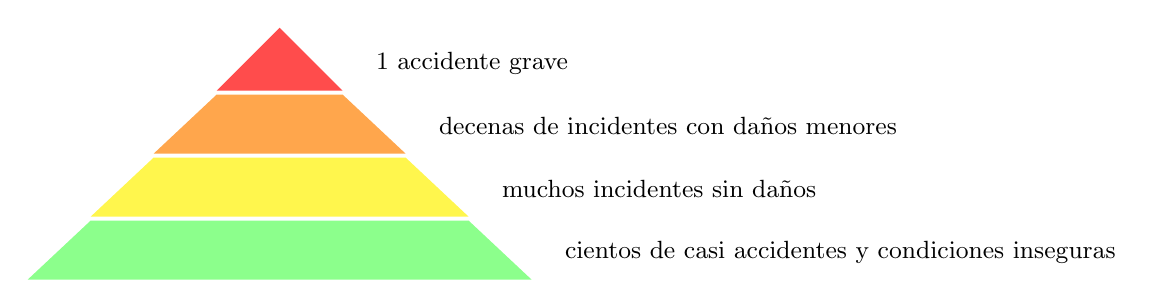
\begin{tikzpicture}[every node/.style={font=\small}]
  \fill[red!70] (0,3.2) -- (-0.8,2.4) -- (0.8,2.4) -- cycle;
  \fill[orange!70] (-0.8,2.35) -- (0.8,2.35) -- (1.6,1.6) -- (-1.6,1.6) -- cycle;
  \fill[yellow!70] (-1.6,1.55) -- (1.6,1.55) -- (2.4,0.8) -- (-2.4,0.8) -- cycle;
  \fill[green!45] (-2.4,0.75) -- (2.4,0.75) -- (3.2,0) -- (-3.2,0) -- cycle;
  \node[anchor=west] at (1.1,2.75) {1 accidente grave};
  \node[anchor=west] at (1.9,1.95) {decenas de incidentes con daños menores};
  \node[anchor=west] at (2.7,1.15) {muchos incidentes sin daños};
  \node[anchor=west] at (3.5,0.35) {cientos de casi accidentes y condiciones inseguras};
\end{tikzpicture}
\end{center}

\subsubsection*{2.2. Enfoque organizacional: el modelo de Reason (``queso suizo'')}
James Reason propuso que los accidentes ocurren cuando se \textbf{alinean los agujeros} de varias
\textbf{defensas} (capas de queso): la organización, la supervisión, las condiciones de trabajo y
las acciones de las personas.
\begin{itemize}
  \item \textbf{Fallas activas:} errores o violaciones de quienes están en contacto directo con la
        aeronave; su efecto es inmediato.
  \item \textbf{Condiciones latentes:} decisiones tomadas lejos del lugar y del momento del
        accidente (presupuestos, turnos, diseño de procedimientos, falta de instrucción) que
        ``esperan'' a que alguien se equivoque.
\end{itemize}

\begin{center}
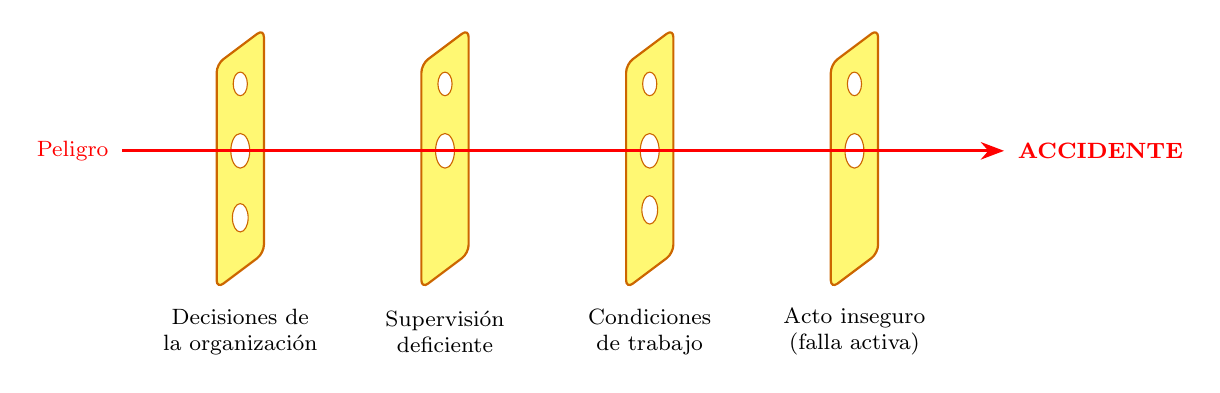
\begin{tikzpicture}[every node/.style={font=\footnotesize, align=center}]
  \foreach \x/\t in {0/Decisiones de\\ la organización, 2.6/Supervisión\\ deficiente,
                     5.2/Condiciones\\ de trabajo, 7.8/Acto inseguro\\ (falla activa)} {
    \fill[yellow!55, draw=orange!80!black, thick, rounded corners=3pt]
      (\x,0) -- (\x+0.6,0.45) -- (\x+0.6,3.3) -- (\x,2.85) -- cycle;
    \node at (\x+0.3,-0.55) {\t};
  }
  \foreach \x in {0,2.6,5.2,7.8} {
    \fill[white, draw=orange!80!black] (\x+0.3,1.75) ellipse (0.12 and 0.22);
    \fill[white, draw=orange!80!black] (\x+0.3,2.6) ellipse (0.09 and 0.15);
  }
  \fill[white, draw=orange!80!black] (0.3,0.9) ellipse (0.1 and 0.18);
  \fill[white, draw=orange!80!black] (5.5,1.0) ellipse (0.1 and 0.18);
  \draw[-{Stealth}, very thick, red] (-1.2,1.75) -- (10.0,1.75);
  \node[red, anchor=west] at (10.05,1.75) {\textbf{ACCIDENTE}};
  \node[red, anchor=east] at (-1.25,1.75) {Peligro};
\end{tikzpicture}
\end{center}

\subsubsection*{2.3. Enfoque sistémico o moderno}
Ve a la aviación como un \textbf{sistema complejo}: personas, tecnología, organizaciones y
regulaciones en interacción. Los accidentes surgen de la combinación de factores normales que, en
conjunto, se vuelven peligrosos, y de la ``deriva'' de las prácticas reales respecto de lo
escrito. Pone el foco en entender cómo el trabajo \textbf{se hace realmente}, en aprender también
de lo que sale bien y en fortalecer la \textbf{resiliencia} de la organización.

\begin{center}
\small
\begin{tabular}{|p{0.22\linewidth}|p{0.33\linewidth}|p{0.33\linewidth}|}
\hline
 & \textbf{Enfoque tradicional} & \textbf{Enfoque moderno} \\ \hline
Pregunta & ¿Quién tuvo la culpa? & ¿Por qué tuvo sentido lo que hicieron? ¿Qué falló en el
sistema? \\ \hline
Causa & Una, la última & Muchas, organizacionales y latentes \\ \hline
Respuesta & Sancionar, reentrenar a la persona & Corregir condiciones, procedimientos y
organización \\ \hline
Información & Se oculta por miedo & Se reporta (cultura justa) \\ \hline
Actuación & Reactiva (después del accidente) & Proactiva y predictiva (antes) \\ \hline
\end{tabular}
\end{center}

% ------------------------------------------------------------
\section*{3. LA INVESTIGACIÓN DE ACCIDENTES}

El \textbf{Anexo 13} de la OACI establece que el \textbf{único objetivo} de la investigación de
accidentes e incidentes es \textbf{prevenir} futuros accidentes, y \textbf{no determinar culpas ni
responsabilidades}. En la Argentina la realiza la \textbf{Junta de Seguridad en el Transporte
(JST)}, independiente de la autoridad que regula (la ANAC) y de la Justicia.

\paragraph*{Etapas.} Notificación del suceso; preservación de las evidencias; trabajo de campo
(restos, registradores de vuelo, documentación, testigos); análisis; informe preliminar;
\textbf{informe final} con conclusiones y \textbf{recomendaciones de seguridad} dirigidas a
quienes pueden corregir el problema (autoridad, fabricante, operador, taller).

\paragraph*{El aporte del mantenimiento.} En toda investigación se revisan los registros de
mantenimiento, el cumplimiento de directivas y la historia de los componentes. Un registro
completo y veraz protege a la aviación y al propio técnico.

% ------------------------------------------------------------
\section*{4. EL CICLO DE LA SEGURIDAD OPERACIONAL Y LA GESTIÓN DE RIESGOS}

\begin{center}
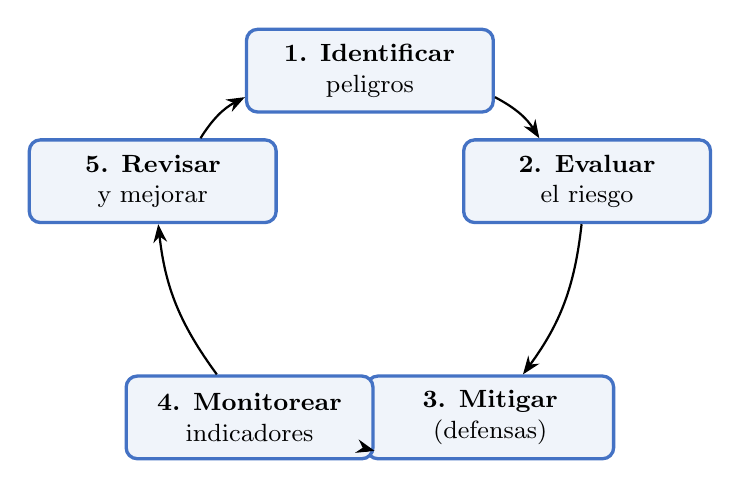
\begin{tikzpicture}[every node/.style={font=\small, align=center},
  e/.style={draw=ppAzul, very thick, rounded corners, fill=ppAzul!8, text width=2.9cm,
  minimum height=1.05cm}]
  \node[e] (a) at (90:2.3) {\textbf{1. Identificar}\\ peligros};
  \node[e] (b) at (18:2.9) {\textbf{2. Evaluar}\\ el riesgo};
  \node[e] (c) at (-54:2.6) {\textbf{3. Mitigar}\\ (defensas)};
  \node[e] (d) at (-126:2.6) {\textbf{4. Monitorear}\\ indicadores};
  \node[e] (f) at (162:2.9) {\textbf{5. Revisar}\\ y mejorar};
  \draw[-{Stealth}, thick] (a) to[bend left=15] (b);
  \draw[-{Stealth}, thick] (b) to[bend left=15] (c);
  \draw[-{Stealth}, thick] (c) to[bend left=15] (d);
  \draw[-{Stealth}, thick] (d) to[bend left=15] (f);
  \draw[-{Stealth}, thick] (f) to[bend left=15] (a);
\end{tikzpicture}
\end{center}

\subsubsection*{4.1. Identificación de peligros}
Fuentes \textbf{reactivas} (análisis de accidentes e incidentes ocurridos), \textbf{proactivas}
(reportes voluntarios, auditorías, inspecciones, encuestas) y \textbf{predictivas} (análisis de
datos para detectar tendencias antes de que ocurra algo).

\subsubsection*{4.2. Evaluación del riesgo: la matriz}
\begin{center}
\small
\begin{tabular}{|p{0.30\linewidth}|c|c|c|c|c|}
\hline
\textbf{Probabilidad} $\backslash$ \textbf{Gravedad} & \textbf{A} Catastrófico & \textbf{B}
Peligroso & \textbf{C} Grave & \textbf{D} Leve & \textbf{E} Insignificante \\ \hline
\textbf{5} Frecuente & \textbf{5A} & \textbf{5B} & \textbf{5C} & 5D & 5E \\ \hline
\textbf{4} Ocasional & \textbf{4A} & \textbf{4B} & 4C & 4D & 4E \\ \hline
\textbf{3} Remoto & \textbf{3A} & 3B & 3C & 3D & \textit{3E} \\ \hline
\textbf{2} Improbable & 2A & 2B & 2C & \textit{2D} & \textit{2E} \\ \hline
\textbf{1} Sumamente improbable & 1A & \textit{1B} & \textit{1C} & \textit{1D} & \textit{1E} \\
\hline
\end{tabular}
\end{center}
\begin{itemize}
  \item \textbf{Intolerable} (en negrita: 5A, 5B, 5C, 4A, 4B, 3A): no se puede operar así; hay que
        detener o mitigar de inmediato.
  \item \textbf{Tolerable} (normal): se acepta solo con medidas de mitigación y aprobación de la
        dirección.
  \item \textbf{Aceptable} (en cursiva): se puede operar; se sigue monitoreando.
\end{itemize}

\subsubsection*{4.3. Mitigación: la jerarquía de controles}
De más a menos eficaz: \textbf{eliminar} el peligro; \textbf{sustituir} por algo menos
peligroso; \textbf{controles de ingeniería} (barandas, protecciones, alarmas); \textbf{controles
administrativos} (procedimientos, capacitación, señalización); \textbf{elementos de protección
personal}.

% ------------------------------------------------------------
\section*{5. EL SISTEMA DE GESTIÓN DE LA SEGURIDAD OPERACIONAL (SMS)}

El \textbf{SMS} (\textit{Safety Management System}) es un enfoque sistemático para gestionar la
seguridad operacional, que incluye la estructura organizacional, las responsabilidades, las
políticas y los procedimientos necesarios. Lo exige el \textbf{Anexo 19} de la OACI a los
operadores, talleres de mantenimiento, organizaciones de diseño y fabricación, centros de
instrucción, proveedores de servicios de tránsito aéreo y aeródromos, \textbf{ajustado a su tamaño
y complejidad}. La guía principal es el \textbf{Doc 9859} de la OACI.

\subsubsection*{5.1. El marco del SMS: 4 componentes y 12 elementos}
\begin{center}
\small
\begin{tabular}{|p{0.30\linewidth}|p{0.60\linewidth}|}
\hline
\textbf{Componente} & \textbf{Elementos} \\ \hline
\textbf{1. Política y objetivos de seguridad operacional} & 1.1 Compromiso de la dirección. \newline
1.2 Obligación de rendición de cuentas y responsabilidades. \newline
1.3 Designación del personal clave de seguridad operacional. \newline
1.4 Coordinación de la planificación de respuesta ante emergencias. \newline
1.5 Documentación del SMS. \\ \hline
\textbf{2. Gestión de riesgos de seguridad operacional} & 2.1 Identificación de peligros. \newline
2.2 Evaluación y mitigación de riesgos. \\ \hline
\textbf{3. Aseguramiento de la seguridad operacional} & 3.1 Observación y medición del
rendimiento en materia de seguridad operacional. \newline
3.2 Gestión del cambio. \newline
3.3 Mejora continua del SMS. \\ \hline
\textbf{4. Promoción de la seguridad operacional} & 4.1 Instrucción y educación. \newline
4.2 Comunicación de la seguridad operacional. \\ \hline
\end{tabular}
\end{center}

\subsubsection*{5.2. Indicadores y metas}
Un SMS se mide con \textbf{indicadores de rendimiento} (SPI), por ejemplo: cantidad de reportes
voluntarios por mes, errores de mantenimiento detectados en inspección, fallas repetitivas,
hallazgos de auditoría abiertos. A cada indicador se le fijan \textbf{metas} (SPT) y niveles de
alerta.

\subsubsection*{5.3. El Programa Estatal de Seguridad Operacional (SSP)}
Así como cada organización tiene su SMS, cada \textbf{Estado} debe tener un \textbf{SSP}: el
conjunto de normas y actividades con las que gestiona la seguridad de toda su aviación civil
(regulación, vigilancia, investigación, promoción) y acepta y supervisa los SMS de las
organizaciones.

\subsubsection*{5.4. La cultura de seguridad}
Ningún sistema funciona sin una \textbf{cultura de seguridad}: una organización donde la gente
\textbf{informa} lo que ve (cultura de reporte), se la trata con \textbf{justicia}, la
organización \textbf{aprende} de sus errores y la dirección da el ejemplo. La seguridad no es un
departamento: es la forma de trabajar de todos.

% ------------------------------------------------------------
\section*{6. LOS COSTOS DE LOS ACCIDENTES Y DE LA SEGURIDAD}

\begin{itemize}
  \item \textbf{Costos directos:} daños a la aeronave, lesiones, indemnizaciones; en general los
        cubre el seguro.
  \item \textbf{Costos indirectos:} los que no cubre el seguro, y suelen ser \textbf{mucho
        mayores} (la ``parte oculta del iceberg''): pérdida de ingresos mientras la aeronave no
        vuela, reemplazo de equipos, horas de investigación y trámites, multas, aumento de las
        primas de seguro, pérdida de clientes y de reputación, efecto en el personal.
  \item \textbf{Costos de los incidentes:} aunque no haya víctimas, un incidente genera
        reparaciones, demoras, cancelaciones y AOG.
  \item \textbf{Costos de la seguridad:} instrucción, personal de calidad y SMS, herramientas,
        repuestos, tiempo de inspección. Son una \textbf{inversión}: previenen pérdidas muy
        superiores.
\end{itemize}
\textit{``Si usted piensa que la seguridad es cara, pruebe con un accidente.''}

% ------------------------------------------------------------
\section*{7. CASOS PARA ANALIZAR}

\begin{center}
\footnotesize
\begin{tabular}{|p{0.22\linewidth}|p{0.40\linewidth}|p{0.28\linewidth}|}
\hline
\textbf{Caso} & \textbf{Qué pasó} & \textbf{Tema clave} \\ \hline
Tenerife (España), 27/3/1977 & Dos Boeing 747 chocaron en la pista con niebla; 583 muertos, el
peor accidente de la historia de la aviación. & Comunicación, jerarquía en cabina, origen del
CRM. \\ \hline
American 191 (Chicago), 25/5/1979 & Un DC-10 perdió un motor al despegar; el pilón había sido
dañado en mantenimiento por un procedimiento no aprobado para ahorrar tiempo. & Procedimientos
``alternativos'', presión de tiempo. \\ \hline
Aloha 243 (Hawái), 28/4/1988 & Un Boeing 737 con muchísimos ciclos perdió parte del techo del
fuselaje en vuelo; murió una tripulante. & Fatiga y corrosión, eficacia de las inspecciones. \\
\hline
Continental Express 2574 (Texas), 11/9/1991 & Trabajo incompleto en el estabilizador no
comunicado en el pase de turno. & Pase de turno, MRM. \\ \hline
British Airways 5390 (R. Unido), 10/6/1990 & Parabrisas instalado con tornillos equivocados. &
Número de parte, verificación. \\ \hline
Austral 2553 (Fray Bentos, Uruguay), 10/10/1997 & Un DC-9 se estrelló tras una indicación
errónea de velocidad por hielo en el sistema pitot y la extensión de los slats a alta velocidad;
74 muertos. & Instrumentos, entrenamiento, factores humanos. \\ \hline
LAPA 3142 (Aeroparque), 31/8/1999 & Un Boeing 737 intentó despegar sin los flaps extendidos; la
alarma sonó y no fue atendida; 65 muertos. & Factores organizacionales, cultura de la empresa
y vigilancia del Estado. \\ \hline
Alaska 261 (California), 31/1/2000 & Un MD-83 perdió el control por el desgaste del tornillo
del estabilizador horizontal, con lubricación insuficiente e intervalos de inspección
extendidos; 88 muertos. & Programa de mantenimiento, intervalos. \\ \hline
Southwest 1380 (EE.\,UU.), 17/4/2018 & Un álabe del fan se rompió por fatiga; los restos dañaron
el fuselaje; murió una pasajera. & Inspecciones de motores, AD. \\ \hline
Alaska 1282 (Portland), 5/1/2024 & En un 737 MAX 9 se desprendió en vuelo un tapón de puerta al
que le faltaban los pernos tras un trabajo en fábrica; sin víctimas fatales. & Control de
calidad, documentación de remociones. \\ \hline
Washington DC, 29/1/2025 & Colisión en vuelo entre un avión regional y un helicóptero militar
cerca del aeropuerto Reagan; 67 muertos. & Gestión del tránsito aéreo, separación, riesgos
conocidos no gestionados. \\ \hline
UPS 2976 (Louisville), 4/11/2025 & Un MD-11F perdió el motor izquierdo con su pilón al despegar;
14 muertos (ver Unidad 2). & Aeronavegabilidad continuada, información del fabricante. \\
\hline
\end{tabular}
\end{center}

\paragraph*{Material audiovisual sugerido.}
\begin{itemize}
  \item La serie documental \textbf{\textit{Mayday: Catástrofes aéreas}} (\textit{Air Crash
        Investigation}), que reconstruye muchos de estos casos con la información de los
        informes oficiales (Tenerife, Aloha 243, Alaska 261, British Airways 5390, entre otros).
  \item La película argentina \textbf{\textit{Whisky Romeo Zulu}} (2004), de Enrique Piñeyro,
        ex piloto de LAPA, sobre el contexto organizacional del accidente de LAPA 3142.
  \item Los \textbf{informes finales} de la JST y de la NTSB, disponibles en sus sitios web.
\end{itemize}

% ------------------------------------------------------------
\section*{8. ACTIVIDADES DE LA UNIDAD}
\begin{enumerate}
  \item \textbf{Tradicional vs.\ moderno:} elegir un caso de la tabla y escribir dos conclusiones:
        una como la escribiría el enfoque tradicional (``la causa fue...'') y otra con el enfoque
        moderno (factores latentes y organizacionales). ¿Cuál previene mejor?
  \item \textbf{Queso suizo:} analizar un caso con el modelo de Reason, identificando las fallas
        activas y las condiciones latentes en cada capa.
  \item \textbf{Informe de la JST:} leer un informe final de la JST de un accidente de aviación
        general y resumir sus recomendaciones de seguridad.
  \item \textbf{Matriz de riesgos del taller:} identificar diez peligros del taller de la escuela,
        evaluarlos en la matriz y proponer medidas según la jerarquía de controles.
  \item \textbf{Simulación del ciclo:} implementar una medida preventiva en el taller (por ejemplo,
        un tablero de sombra para herramientas) y medir durante un mes un indicador.
  \item \textbf{Informe de costos:} con un caso hipotético de un incidente de mantenimiento (por
        ejemplo, una herramienta olvidada que dañó un motor), estimar los costos directos e
        indirectos y redactar un informe que justifique la inversión en prevención.
\end{enumerate}
      % Unidad 6: prevención de accidentes y SMS
% ============================================================
% UNIDAD 7: OPERACIONES AÉREAS, ESPACIO AÉREO Y CARTAS
% ============================================================
\clearpage
\section*{UNIDAD 7: OPERACIONES AÉREAS}
\subsection*{Tipos de operación, espacio aéreo y cartas aeronáuticas}

\begin{recuadro}
\textbf{Objetivo de la unidad:} conocer cómo se organizan las operaciones aéreas, cómo se divide y
controla el espacio aéreo y cómo se leen las cartas aeronáuticas, para entender el entorno en el
que funcionan los equipos de comunicaciones, navegación y vigilancia que mantiene el técnico
aviónico.
\end{recuadro}

% ------------------------------------------------------------
\section*{1. TIPOS DE OPERACIÓN}

\begin{center}
\small
\begin{tabular}{|p{0.30\linewidth}|p{0.14\linewidth}|p{0.44\linewidth}|}
\hline
\textbf{Tipo} & \textbf{Norma} & \textbf{Ejemplos} \\ \hline
Aviación general & RAAC 91 & Vuelos privados, aeroclubes, instrucción, aviación corporativa. \\
\hline
Transporte aéreo regular & RAAC 121 & Líneas aéreas con aviones grandes. \\ \hline
Transporte no regular y operaciones menores & RAAC 135 & Taxis aéreos, ambulancias aéreas,
vuelos ejecutivos. \\ \hline
Trabajo aéreo & RAAC 137 & Aviación agrícola, fotografía, inspección de líneas eléctricas. \\
\hline
Aeronaves pilotadas a distancia & RAAC 100 & Drones (RPAS). \\ \hline
Aviación de Estado & -- & Militar, policial, sanitaria oficial (matrícula LQ). \\ \hline
\end{tabular}
\end{center}

\paragraph*{Reglas de vuelo.}
\begin{itemize}
  \item \textbf{VFR} (reglas de vuelo visual): el piloto se separa de otras aeronaves y del
        terreno mirando hacia afuera. Requiere condiciones meteorológicas visuales (VMC).
  \item \textbf{IFR} (reglas de vuelo por instrumentos): se vuela con referencia a los
        instrumentos y siguiendo procedimientos y autorizaciones del control de tránsito. Es la
        regla de la aviación comercial, y la que exige que la aviónica de navegación y
        comunicaciones funcione con total confiabilidad.
\end{itemize}

% ------------------------------------------------------------
\section*{2. LOS SERVICIOS DE TRÁNSITO AÉREO}

En la Argentina los presta la \textbf{EANA}. Incluyen:
\begin{itemize}
  \item \textbf{Control de tránsito aéreo (ATC):} \textbf{torre de control} (TWR) para el aeródromo
        y sus inmediaciones; \textbf{control de aproximación} (APP) para las llegadas y salidas; y
        \textbf{centro de control de área} (ACC) para la fase en ruta.
  \item \textbf{Servicio de información de vuelo} (FIS): datos útiles para la seguridad del vuelo.
  \item \textbf{Servicio de alerta}: notifica a búsqueda y salvamento cuando una aeronave necesita
        ayuda.
\end{itemize}
Para prestarlos, el espacio aéreo argentino se divide en \textbf{regiones de información de vuelo}
(FIR), cada una con su centro de control de área.

\paragraph*{El transpondedor.} Es el equipo de a bordo que responde a los radares secundarios
con un código de cuatro dígitos asignado por el control. Algunos códigos son universales:
\textbf{7500} (interferencia ilícita), \textbf{7600} (falla de comunicaciones) y \textbf{7700}
(emergencia). Con \textbf{ADS-B}, la aeronave además transmite su posición GPS, su altitud y su
velocidad.

% ------------------------------------------------------------
\section*{3. EL ESPACIO AÉREO}

\subsubsection*{3.1. Espacios aéreos controlados y no controlados}
\begin{itemize}
  \item \textbf{Zona de control (CTR):} rodea a un aeródromo controlado, desde el suelo hasta un
        límite superior.
  \item \textbf{Área de control terminal (TMA):} encima y alrededor de una o varias CTR, para
        ordenar llegadas y salidas.
  \item \textbf{Aerovías (AWY):} ``rutas'' del cielo, con ancho y altitudes definidos, que unen
        radioayudas o puntos de notificación.
  \item \textbf{Espacios reglamentados:} \textbf{prohibidos} (no se puede volar),
        \textbf{restringidos} (solo con condiciones) y \textbf{peligrosos} (hay actividades de
        riesgo, como tiro o vuelo de práctica militar).
\end{itemize}

\subsubsection*{3.2. Clases de espacio aéreo (OACI)}
\begin{center}
\small
\begin{tabular}{|c|p{0.18\linewidth}|p{0.64\linewidth}|}
\hline
\textbf{Clase} & \textbf{Vuelos permitidos} & \textbf{Servicio} \\ \hline
A & Solo IFR & Todos controlados y separados entre sí. \\ \hline
B & IFR y VFR & Todos controlados y separados entre sí. \\ \hline
C & IFR y VFR & IFR separados de todos; VFR separados de IFR y con información de otros VFR. \\
\hline
D & IFR y VFR & IFR separados de IFR; todos reciben información de tránsito. \\ \hline
E & IFR y VFR & IFR controlados y separados de IFR; VFR no controlados. \\ \hline
F & IFR y VFR & Asesoramiento de tránsito para IFR (no controlado). \\ \hline
G & IFR y VFR & No controlado; solo información de vuelo. \\ \hline
\end{tabular}
\end{center}

% ------------------------------------------------------------
\section*{4. LAS CARTAS AERONÁUTICAS}

Las cartas aeronáuticas se rigen por el \textbf{Anexo 4} de la OACI y se publican, junto con toda la
información oficial para volar en el país, en la \textbf{AIP} (Publicación de Información
Aeronáutica) de la Argentina. Los cambios temporarios se informan por \textbf{NOTAM} (aviso a los
aviadores): por ejemplo, una radioayuda fuera de servicio por mantenimiento.

\begin{center}
\small
\begin{tabular}{|p{0.32\linewidth}|p{0.58\linewidth}|}
\hline
\textbf{Carta} & \textbf{Para qué sirve} \\ \hline
Carta aeronáutica visual (escala 1:500.000 o 1:1.000.000) & Vuelo VFR: relieve, ciudades, rutas,
ríos, aeródromos, espacios aéreos. \\ \hline
Carta de navegación en ruta (ENR) & Vuelo IFR: aerovías, radioayudas, altitudes mínimas, límites
de FIR. \\ \hline
Salidas y llegadas normalizadas (SID y STAR) & Procedimientos para salir de un aeródromo y para
llegar a él. \\ \hline
Carta de aproximación por instrumentos (IAC) & Procedimiento para aproximarse y aterrizar con
ILS, VOR, RNAV (GPS). \\ \hline
Plano de aeródromo (ADC) & Pistas, calles de rodaje, plataformas, frecuencias. \\ \hline
\end{tabular}
\end{center}

\subsubsection*{4.1. Qué se lee en una carta}
\begin{itemize}
  \item \textbf{Coordenadas} (latitud y longitud), escala y proyección.
  \item \textbf{Rumbos} magnéticos y la \textbf{declinación magnética} (diferencia entre el norte
        verdadero y el magnético).
  \item \textbf{Radioayudas}, con su símbolo, nombre, identificación en código Morse y
        \textbf{frecuencia}: \textbf{VOR} (VHF, 108 a 117,95 MHz), \textbf{DME} (distancia),
        \textbf{NDB} (baja/media frecuencia), \textbf{ILS} (localizador y senda de planeo).
  \item \textbf{Altitudes mínimas} de las rutas y del terreno.
  \item \textbf{Frecuencias de comunicaciones} de torre, aproximación y control.
  \item \textbf{Espacios aéreos} con sus clases y límites verticales.
\end{itemize}

\begin{recuadro}
\textbf{¿Por qué le importa al técnico aviónico?} Cada símbolo de la carta es un sistema que el
técnico mantiene o del que depende un equipo de a bordo: el receptor VOR/ILS, el DME, el ADF, el
GPS, el transpondedor y las radios de VHF. Entender cómo los usa el piloto ayuda a diagnosticar
una falla reportada (``el VOR 1 marca 5 grados de diferencia con el VOR 2'') y a dimensionar su
impacto en la operación y en la lista de equipo mínimo (MEL).
\end{recuadro}

% ------------------------------------------------------------
\section*{5. ACTIVIDADES DE LA UNIDAD}
\begin{enumerate}
  \item \textbf{Lectura de cartas:} con una carta visual y una de aproximación de un aeródromo
        cercano (por ejemplo, Aeroparque, Ezeiza o San Fernando), identificar radioayudas,
        frecuencias, espacios aéreos y altitudes mínimas.
  \item \textbf{NOTAM:} buscar NOTAM vigentes de un aeródromo y explicar cuáles afectan equipos de
        navegación o comunicaciones.
  \item \textbf{De la carta al equipo:} para una aproximación ILS, listar todos los equipos de a
        bordo y de tierra que intervienen y qué pasaría si fallara cada uno.
  \item \textbf{Clases de espacio:} para tres vuelos (un VFR de aeroclub, un vuelo de línea, un
        drone), indicar en qué espacios pueden volar y qué necesitan.
\end{enumerate}
    % Unidad 7: operaciones aéreas, espacio aéreo y cartas
% ============================================================
% PROYECTO INTEGRADOR: SMS DEL TALLER DE AVIÓNICA
% ============================================================
\clearpage
\section*{PROYECTO INTEGRADOR}
\subsection*{Sistema de Gestión de la Seguridad Operacional del taller de aviónica}

\begin{recuadro}
\textbf{Consigna general:} diseñar e implementar, durante el segundo cuatrimestre, un
\textbf{SMS simplificado} para el taller de aviónica de la escuela, siguiendo los cuatro
componentes del Anexo 19 de la OACI, adaptado al tamaño y a la complejidad del taller.

\textbf{Modalidad:} trabajo en equipos con roles. \textbf{Entrega final:} Manual SMS del taller,
registro de peligros y matriz de riesgos, sistema de reportes funcionando, tablero de indicadores
y presentación oral ante la dirección de la escuela.
\end{recuadro}

% ------------------------------------------------------------
\section*{1. ORGANIZACIÓN}
\begin{center}
\small
\begin{tabular}{|p{0.28\linewidth}|p{0.62\linewidth}|}
\hline
\textbf{Equipo} & \textbf{Responsabilidad} \\ \hline
Política y documentación & Redactar la política de seguridad, definir roles y armar el Manual
SMS. \\ \hline
Gestión de riesgos & Identificar peligros, evaluarlos en la matriz y proponer mitigaciones. \\
\hline
Reportes e investigación & Diseñar el sistema de reportes voluntarios e investigar los sucesos
con el método MEDA. \\ \hline
Aseguramiento & Definir indicadores, metas, auditorías internas y gestión del cambio. \\ \hline
Promoción & Capacitar a otros cursos, publicar un boletín de seguridad mensual y la cartelería. \\
\hline
\end{tabular}
\end{center}
El \textbf{comité de seguridad operacional} reúne a un representante de cada equipo y al docente
(que actúa como responsable del SMS), y se reúne cada quince días.

% ------------------------------------------------------------
\section*{2. ETAPAS}

\subsubsection*{Etapa 1. Política y objetivos (Componente 1)}
\begin{itemize}
  \item Redactar la \textbf{política de seguridad operacional} del taller (una página): compromiso,
        cultura justa, obligación de reportar, objetivos. Firmada por la dirección o el jefe de
        taller.
  \item Definir responsabilidades: quién es responsable del SMS, qué hace cada estudiante y cada
        docente.
  \item Elaborar el \textbf{plan de respuesta ante emergencias} del taller: incendio,
        electrocución, accidente con herramientas, evacuación; números de emergencia, ubicación de
        matafuegos, botiquín y DEA.
\end{itemize}

\subsubsection*{Etapa 2. Gestión de riesgos (Componente 2)}
\begin{itemize}
  \item Recorrer el taller y armar el \textbf{registro de peligros} (mínimo 15).
  \item Evaluar cada uno en la \textbf{matriz de riesgos} y proponer medidas con la jerarquía de
        controles.
\end{itemize}

\begin{center}
\footnotesize
\setlength{\tabcolsep}{3pt}
\newcolumntype{L}[1]{>{\raggedright\arraybackslash}p{#1\linewidth}}
\begin{tabular}{|c|L{0.21}|L{0.17}|c|L{0.21}|L{0.08}|L{0.11}|}
\hline
\textbf{N°} & \textbf{Peligro} & \textbf{Consecuencia} & \textbf{Riesgo} & \textbf{Mitigación} &
\textbf{Riesgo resid.} & \textbf{Respons.} \\ \hline
1 & Fuente de 28 V DC sin protección en el banco & Descarga, quemadura, daño a equipos & 3C &
Tapas protectoras, bloqueo y etiquetado & 2D & Equipo 2 \\ \hline
2 & Herramientas sin control al terminar la clase & Herramienta olvidada dentro de un equipo
(FOD) & 4C & Tablero de sombra y conteo final & 2D & Pañol \\ \hline
3 & & & & & & \\ \hline
4 & & & & & & \\ \hline
\end{tabular}
\end{center}

\subsubsection*{Etapa 3. Aseguramiento (Componente 3)}
\begin{itemize}
  \item Definir al menos \textbf{cuatro indicadores} (SPI) con su meta, por ejemplo: reportes
        voluntarios por mes; herramientas faltantes al cierre de la clase; equipos devueltos con
        falla al pañol; hallazgos de la auditoría interna resueltos.
  \item Hacer una \textbf{auditoría interna} del taller con una lista de verificación.
  \item Aplicar la \textbf{gestión del cambio} a una novedad real (un equipo nuevo, un cambio de
        aula, un nuevo procedimiento): ¿qué peligros nuevos aparecen?
\end{itemize}

\subsubsection*{Etapa 4. Promoción (Componente 4)}
\begin{itemize}
  \item Dar una \textbf{capacitación} de 40 minutos a un curso menor sobre la docena sucia y el
        sistema de reportes.
  \item Publicar un \textbf{boletín de seguridad} mensual con los reportes recibidos (sin nombres),
        las lecciones aprendidas y los indicadores.
\end{itemize}

% ------------------------------------------------------------
\section*{3. FORMULARIO DE REPORTE VOLUNTARIO}
{\small
\renewcommand{\arraystretch}{1.5}
\begin{tabular}{|p{0.955\linewidth}|}
\hline
\textbf{REPORTE VOLUNTARIO DE SEGURIDAD OPERACIONAL -- TALLER DE AVIÓNICA} \hfill N°: \makebox[2cm]{\dotfill} \\ \hline
Fecha y hora del suceso: \dotfill \quad Lugar: \makebox[4.5cm]{\dotfill} \\ \hline
Tipo: \casilla\ Peligro \quad \casilla\ Error o casi accidente \quad \casilla\ Incidente \quad
\casilla\ Sugerencia \\ \hline
¿Qué pasó o qué observó? \\[1.6cm] \hline
¿Por qué cree que pasó? \\[1.2cm] \hline
¿Qué propone para que no vuelva a pasar? \\[1.2cm] \hline
Nombre (optativo): \dotfill \quad \casilla\ Deseo recibir respuesta \\ \hline
\textit{Este reporte es confidencial. Su objetivo es aprender y prevenir, no sancionar.} \\ \hline
\end{tabular}
}

% ------------------------------------------------------------
\section*{4. ENTREGABLES Y EVALUACIÓN}
\begin{center}
\small
\begin{tabular}{|p{0.66\linewidth}|c|}
\hline
\textbf{Entregable} & \textbf{Peso} \\ \hline
Política de seguridad, roles y plan de respuesta ante emergencias & 15\% \\ \hline
Registro de peligros y matriz de riesgos con mitigaciones & 25\% \\ \hline
Sistema de reportes funcionando e investigación MEDA de al menos un suceso & 20\% \\ \hline
Indicadores, auditoría interna y gestión del cambio & 15\% \\ \hline
Capacitación y boletín de seguridad & 10\% \\ \hline
Manual SMS completo y presentación oral & 15\% \\ \hline
\end{tabular}
\end{center}

\begin{recuadro}
\textbf{Para el CV:} al terminar, cada estudiante puede incluir en su currículum la experiencia
de \textit{``Diseño e implementación de un Sistema de Gestión de la Seguridad Operacional (SMS)
según el Anexo 19 de la OACI en un taller de aviónica''}, junto con las tareas concretas que
realizó en su equipo.
\end{recuadro}
      % Proyecto integrador: SMS del taller de la escuela
\end{document}
